\chapter{Pro Git --- extraits}
\label{chap:git}

\begingroup
\setkeys{Gin}{width=0.6\textwidth}
\raggedbottom

{%
  \itshape%
  Cette annexe contient le chapitre 1 en entier (à l'exception de la
  section 1.5) et des extraits des chapitres 2 (sections 2.1 à 2.5) et
  3 (sections 3.1 à 3.3) de \emph{Pro Git} de \citet{ProGit:2e:2014}.
  Hormis l'adaptation à la mise en page du présent document, la
  conversion des chapitres en sections et des modifications visant à
  corriger les dépassements de texte dans la marge, je n'ai apporté
  aucun changement au texte.

  \emph{Pro Git} est mis à disposition selon le contrat
  \href{http://creativecommons.org/licenses/by-sa/4.0/deed.fr}{%
    Attribution-Pas d’utilisation commerciale-Partage dans les mêmes
    conditions 3.0 non transposé} de Creative Commons. %
}

\section{Démarrage rapide}
\label{sec:git:getting_started}

Ce chapitre traite du démarrage rapide avec Git.
Nous commencerons par expliquer les bases de la gestion de version, puis nous parlerons de l'installation de Git sur votre système et finalement du paramétrage pour commencer à l'utiliser.
À la fin de ce chapitre vous devriez en savoir assez pour comprendre pourquoi on parle beaucoup de Git, pourquoi vous devriez l'utiliser et vous devriez en avoir une installation prête à l'emploi.

\subsection{À propos de la gestion de version}

Qu'est-ce que la gestion de version et pourquoi devriez-vous vous en soucier ?
Un gestionnaire de version est un système qui enregistre l'évolution d'un fichier ou d'un ensemble de fichiers au cours du temps de manière à ce qu'on puisse rappeler une version antérieure d'un fichier à tout moment.
Dans les exemples de ce livre, nous utiliserons des fichiers sources de logiciel comme fichiers sous gestion de version, bien qu'en réalité on puisse l'utiliser avec pratiquement tous les types de fichiers d'un ordinateur.

Si vous êtes un dessinateur ou un développeur web, et que vous voulez conserver toutes les versions d'une image ou d'une mise en page (ce que vous souhaiteriez assurément), un système de gestion de version (VCS en anglais pour \emph{Version Control System}) est un outil qu'il est très sage d'utiliser.
Il vous permet de ramener un fichier à un état précédent, de ramener le projet complet à un état précédent, de visualiser les changements au cours du temps, de voir qui a modifié quelque chose qui pourrait causer un problème, qui a introduit un problème et quand, et plus encore.
Utiliser un VCS signifie aussi généralement que si vous vous trompez ou que vous perdez des fichiers, vous pouvez facilement revenir à un état stable.
De plus, vous obtenez tous ces avantages avec peu de travail additionnel.

\subsubsection{Les systèmes de gestion de version locaux}

La méthode courante pour la gestion de version est généralement de recopier les fichiers dans un autre répertoire (peut-être avec un nom incluant la date dans le meilleur des cas).
Cette méthode est la plus courante parce que c'est la plus simple, mais c'est aussi la moins fiable.
Il est facile d'oublier le répertoire dans lequel vous êtes et d'écrire accidentellement dans le mauvais fichier ou d'écraser des fichiers que vous vouliez conserver.

Pour traiter ce problème, les programmeurs ont développé il y a longtemps des VCS locaux qui utilisaient une base de données simple pour conserver les modifications d'un fichier.

\begin{figure}[H]
  \centering
  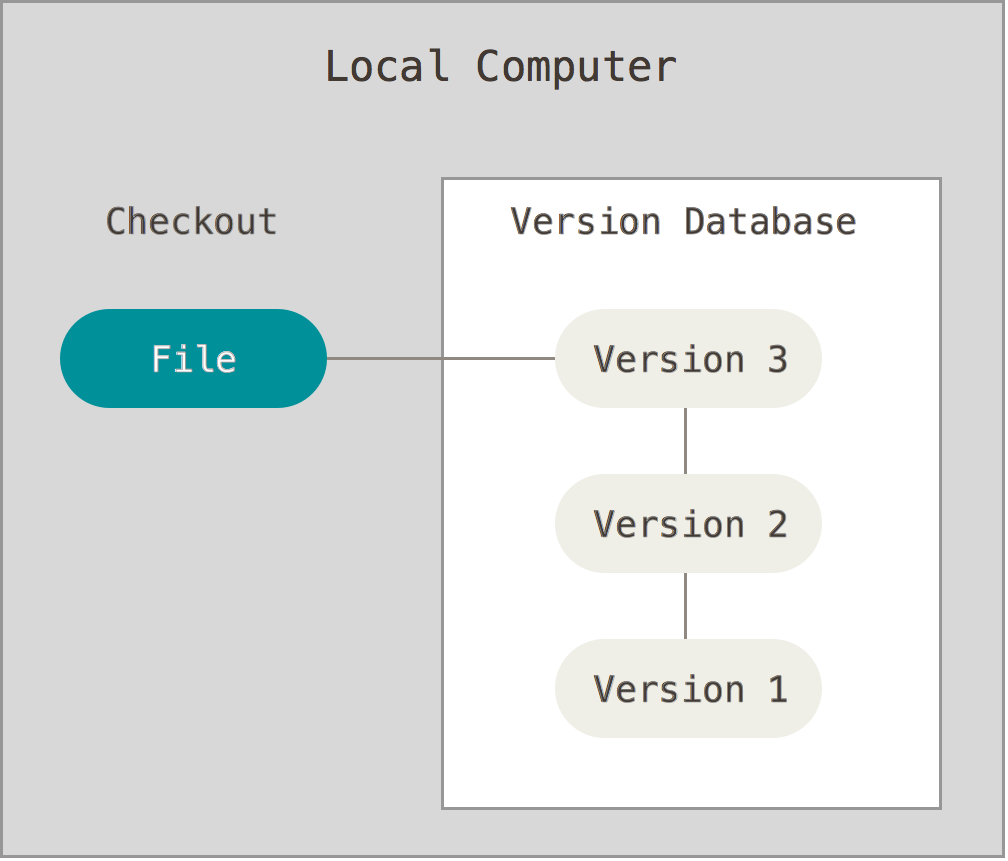
\includegraphics{images/local}
  \caption{Gestion de version locale}
  \label{fig:git:local}
\end{figure}

Un des systèmes les plus populaires était RCS, qui est encore distribué avec de nombreux systèmes d'exploitation aujourd'hui.
Même le système d'exploitation populaire Mac OS X inclut le programme `rcs` lorsqu'on installe les outils de développement logiciel.
Cet outil fonctionne en conservant des ensembles de patchs (c'est-à-dire la différence entre les fichiers) d'une version à l'autre dans un format spécial sur disque ;
il peut alors restituer l'état de n'importe quel fichier à n'importe quel instant en ajoutant toutes les différences.

\subsubsection{Les systèmes de gestion de version centralisés}


Le problème majeur que les gens rencontrent est qu'ils ont besoin de collaborer avec des développeurs sur d'autres ordinateurs.
Pour traiter ce problème, les systèmes de gestion de version centralisés (CVCS en anglais pour \emph{Centralized Version Control Systems}) furent développés.
Ces systèmes tels que CVS, Subversion, et Perforce, mettent en place un serveur central qui contient tous les fichiers sous gestion de version, et des clients qui peuvent extraire les fichiers de ce dépôt central.
Pendant de nombreuses années, cela a été le standard pour la gestion de version.

\begin{figure}[H]
  \centering
  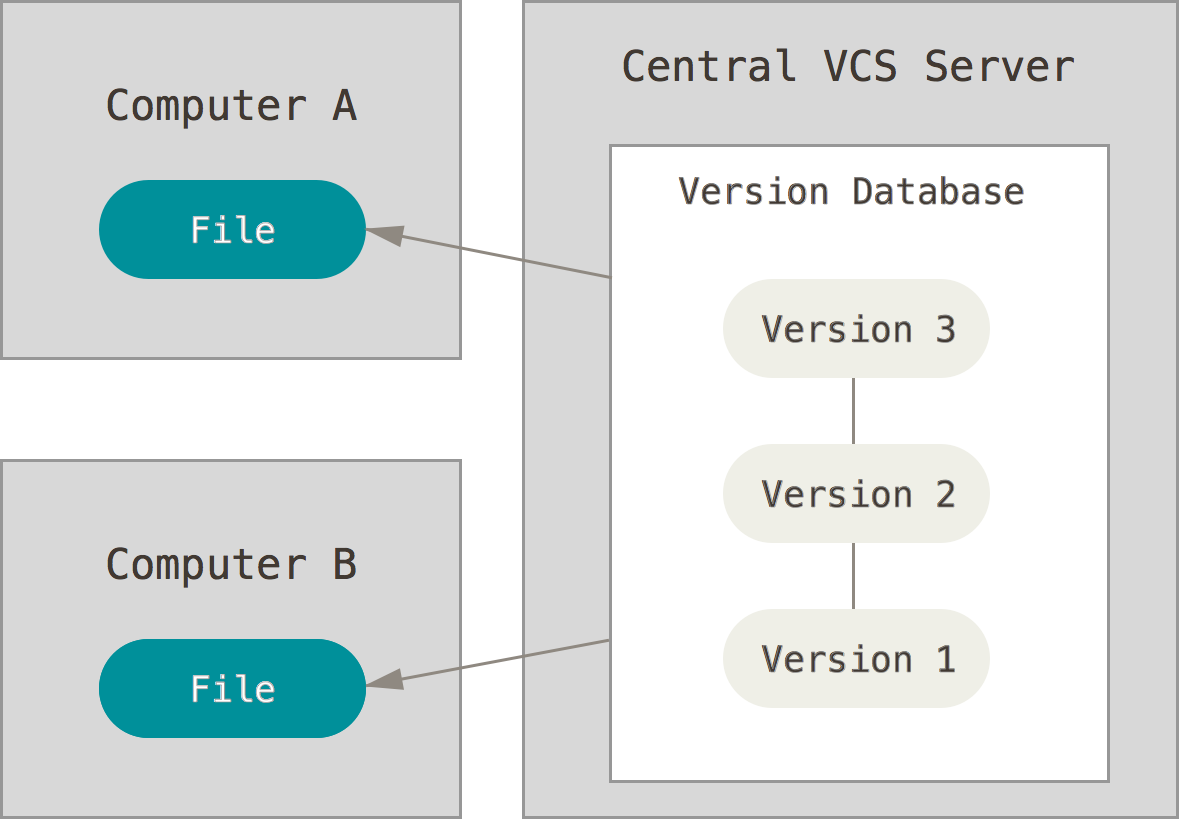
\includegraphics{images/centralized}
  \caption{Gestion de version centralisée}
  \label{fig:git:centralized}
\end{figure}

Ce schéma offre de nombreux avantages par rapport à la gestion de version locale.
Par exemple, chacun sait jusqu'à un certain point ce que tous les autres sont en train de faire sur le projet.
Les administrateurs ont un contrôle fin des permissions et il est beaucoup plus facile d'administrer un CVCS que de gérer des bases de données locales.

Cependant ce système a aussi de nombreux défauts.
Le plus visible est le point unique de panne que le serveur centralisé représente.
Si ce serveur est en panne pendant une heure, alors durant cette heure, aucun client ne peut collaborer ou enregistrer les modifications issues de son travail.
Si le disque dur du serveur central se corrompt, et s'il n'y a pas eu de sauvegarde, vous perdez absolument tout de l'historique d'un projet en dehors des sauvegardes locales que les gens auraient pu réaliser sur leurs machines locales.
Les systèmes de gestion de version locaux souffrent du même problème  --- dès qu'on a tout l'historique d'un projet sauvegardé à un endroit unique, on prend le risque de tout perdre.

\subsubsection{Les systèmes de gestion de version distribués}

C'est à ce moment que les systèmes de gestion de version distribués entrent en jeu (DVCS en anglais pour \emph{Distributed Version Control Systems}).
Dans un DVCS (tel que Git, Mercurial, Bazaar ou Darcs), les clients n'extraient plus seulement la dernière version d'un fichier, mais ils dupliquent complètement le dépôt.
Ainsi, si le serveur disparaît et si les systèmes collaboraient via ce serveur, n'importe quel dépôt d'un des clients peut être copié sur le serveur pour le restaurer.
Chaque extraction devient une sauvegarde complète de toutes les données.

\begin{figure}[H]
  \centering
  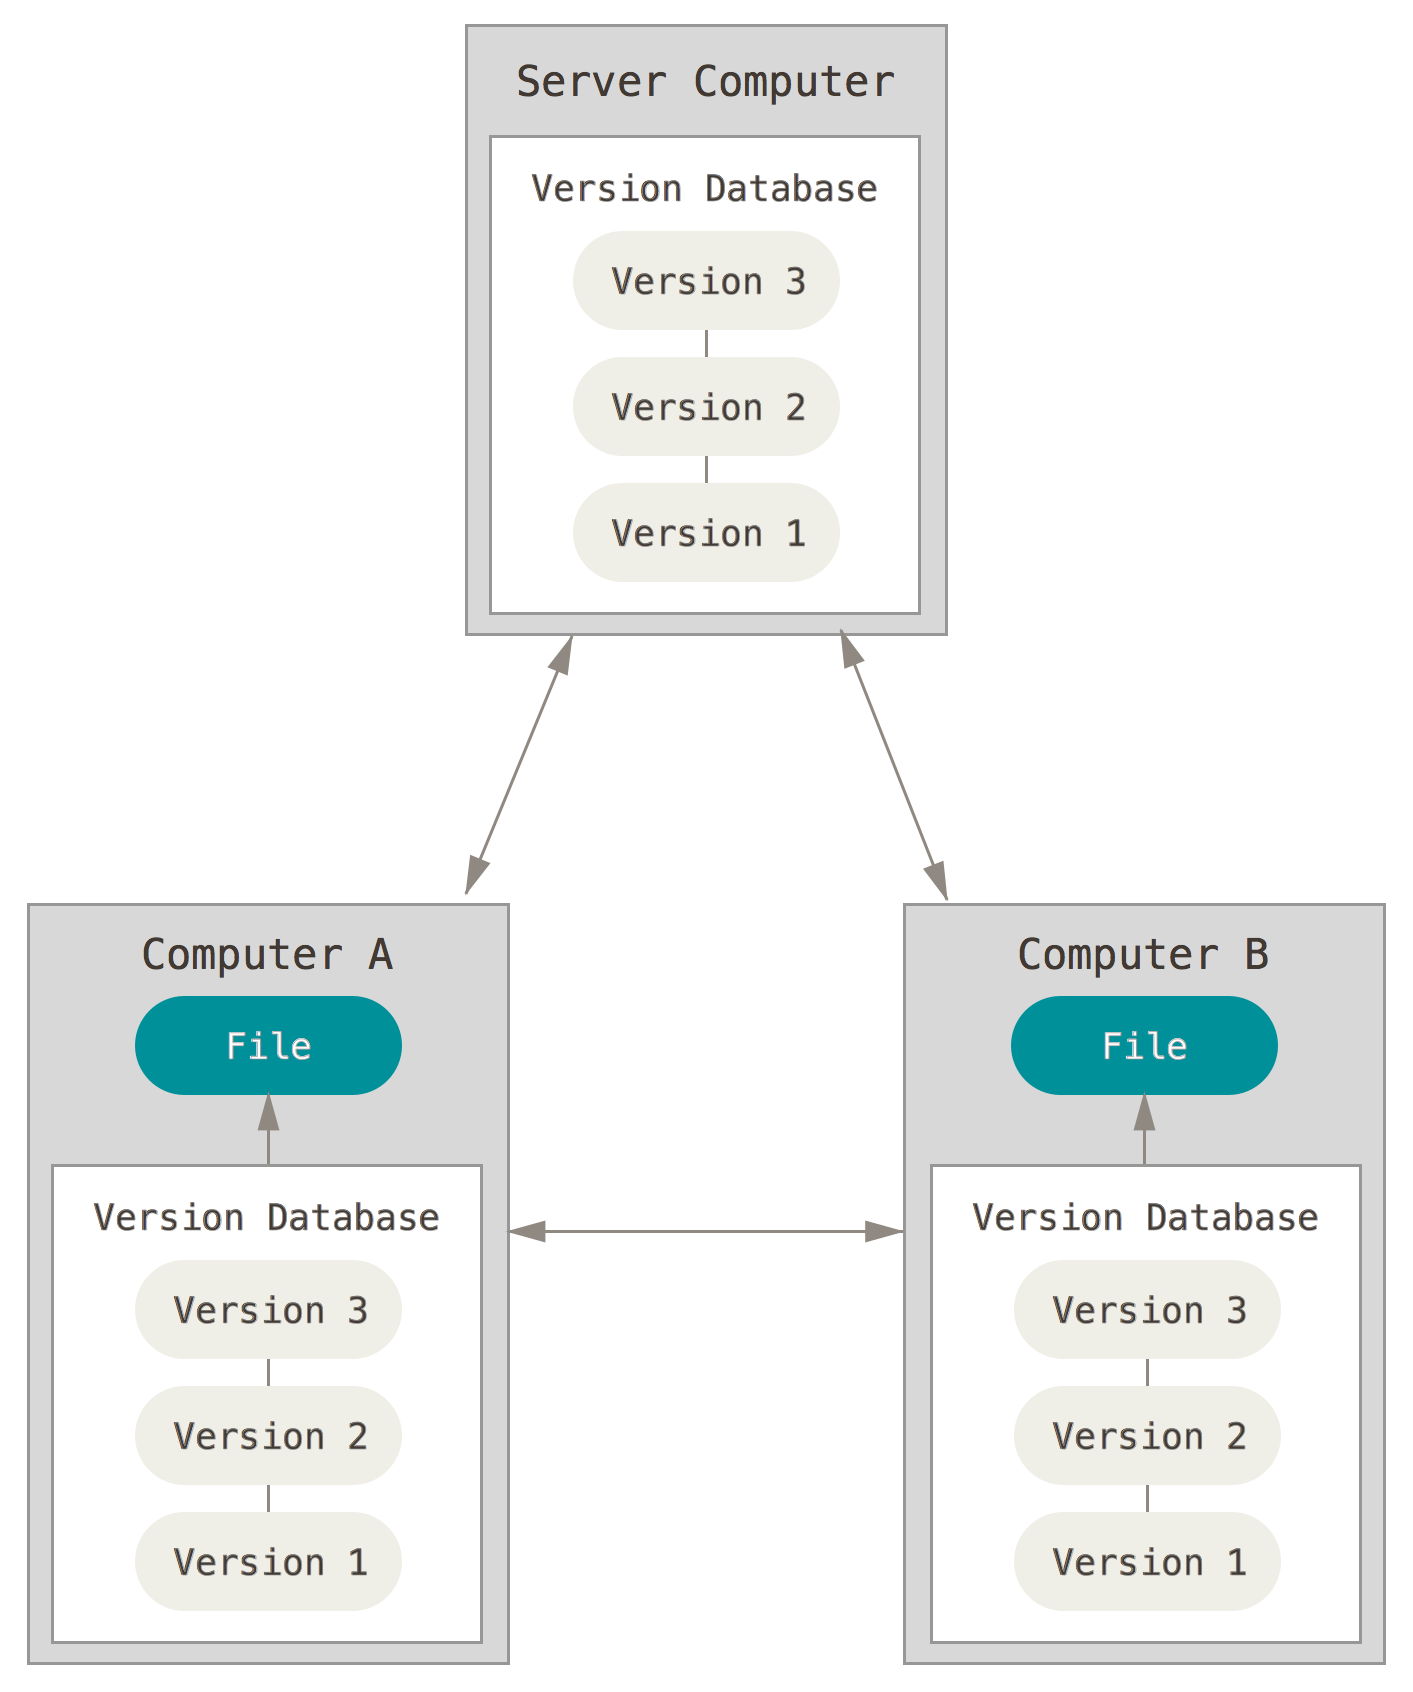
\includegraphics[width=0.5\textwidth,keepaspectratio]{images/distributed}
  \caption{Gestion de version distribuée}
  \label{fig:git:distributed}
\end{figure}

De plus, un grand nombre de ces systèmes gère particulièrement bien le fait d'avoir plusieurs dépôts avec lesquels travailler, vous permettant de collaborer avec différents groupes de personnes de manières différentes simultanément dans le même projet.
Cela permet la mise en place de différentes chaînes de traitement qui ne sont pas réalisables avec les systèmes centralisés, tels que les modèles hiérarchiques.

\subsection{Une rapide histoire de Git}

Comme de nombreuses choses extraordinaires de la vie, Git est né avec une dose de destruction créative et de controverse houleuse.
Le noyau Linux est un projet libre de grande envergure.
Pour la plus grande partie de sa vie (1991–2002), les modifications étaient transmises sous forme de patchs et d'archives de fichiers.
En 2002, le projet du noyau Linux commença à utiliser un DVCS propriétaire appelé BitKeeper.

En 2005, les relations entre la communauté développant le noyau Linux et la société en charge du développement de BitKeeper furent rompues, et le statut de gratuité de l'outil fut révoqué.
Cela poussa la communauté du développement de Linux (et plus particulièrement Linus Torvalds, le créateur de Linux) à développer son propre outil en se basant sur les leçons apprises lors de l'utilisation de BitKeeper.
Certains des objectifs du nouveau système étaient les suivants :

\begin{itemize}
\item vitesse ;
\item conception simple ;
\item support pour les développements non linéaires (milliers de branches parallèles) ;
\item complètement distribué ;
\item capacité à gérer efficacement des projets d'envergure tels que le noyau Linux (vitesse et compacité des données)
\end{itemize}

Depuis sa naissance en 2005, Git a évolué et mûri pour être facile à utiliser tout en conservant ses qualités initiales.
Il est incroyablement rapide, il est très efficace pour de grands projets et il a un incroyable système de branches pour des développements non linéaires (voir la \autoref{sec:git:branching}).

\subsection{Rudiments de Git}

Donc, qu'est-ce que Git en quelques mots ?
Il est important de bien comprendre cette section, parce que si on comprend la nature de Git et les principes sur lesquels il repose, alors utiliser efficacement Git devient simple.
Au cours de l'apprentissage de Git, essayez de libérer votre esprit de ce que vous pourriez connaître d'autres VCS, tels que Subversion et Perforce ;
ce faisant, vous vous éviterez de petites confusions à l'utilisation de cet outil.
Git enregistre et gère l'information très différemment des autres systèmes, même si l'interface utilisateur paraît similaire ;
comprendre ces différences vous évitera des surprises.

\subsubsection{Des instantanés, pas des différences}

La différence majeure entre Git et les autres VCS (Subversion et autres) réside dans la manière dont Git considère les données.
Au niveau conceptuel, la plupart des autres systèmes gèrent l'information comme une liste de modifications de fichiers.
Ces systèmes (CVS, Subversion, Perforce, Bazaar et autres) considèrent l'information qu'ils gèrent comme une liste de fichiers et les modifications effectuées sur chaque fichier dans le temps.

\begin{figure}[H]
  \centering
  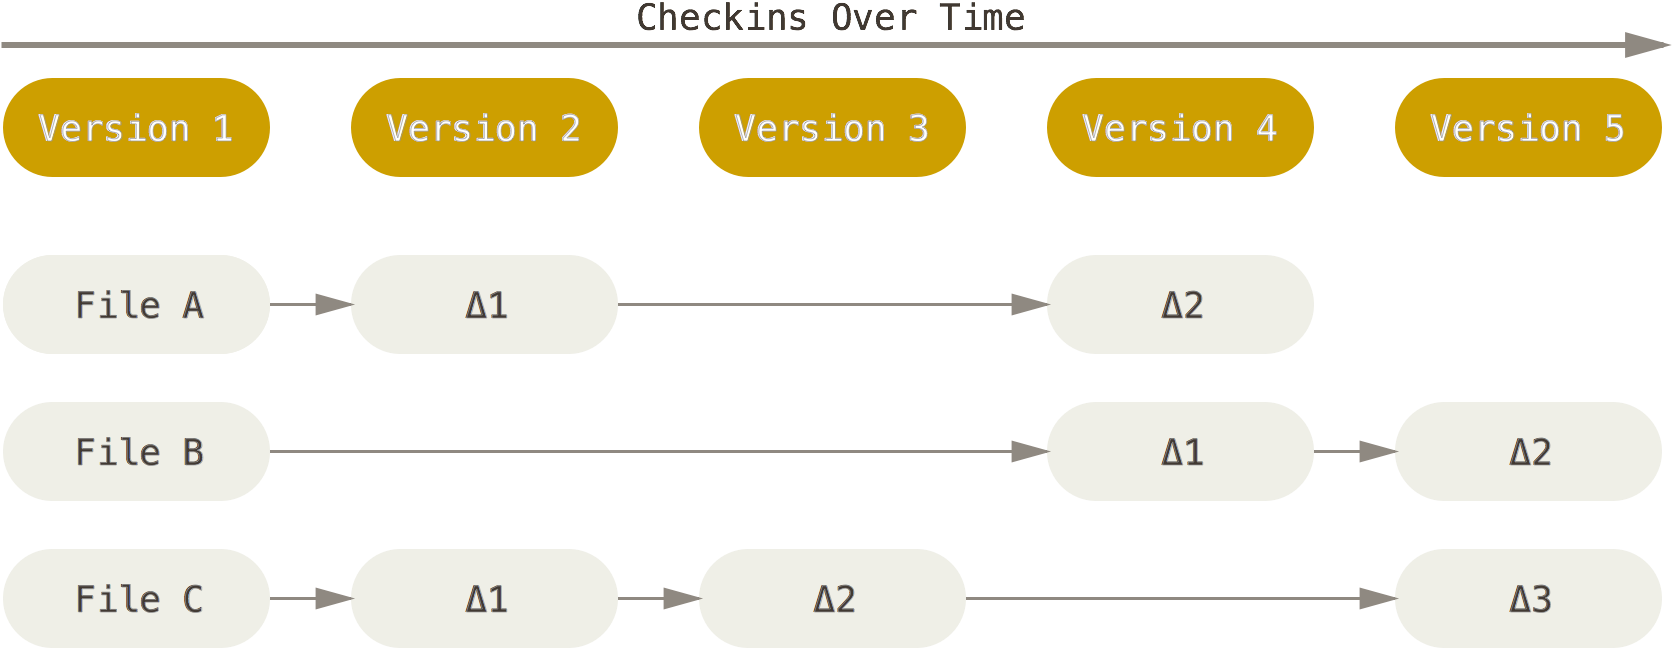
\includegraphics{images/deltas}
  \caption{D'autres systèmes sauvent l'information comme des modifications sur des fichiers}
  \label{fig:git:deltas}
\end{figure}

Git ne gère pas et ne stocke pas les informations de cette manière.
À la place, Git pense ses données plus comme un instantané d'un mini système de fichiers.
À chaque fois que vous validez ou enregistrez l'état du projet dans Git, il prend effectivement un instantané du contenu de votre espace de travail à ce moment et enregistre une référence à cet instantané.
Pour être efficace, si les fichiers n'ont pas changé, Git ne stocke pas le fichier à nouveau, juste une référence vers le fichier original qu'il a déjà enregistré.
Git pense ses données plus à la manière d'un *flux d'instantanés*.

\begin{figure}[H]
  \centering
  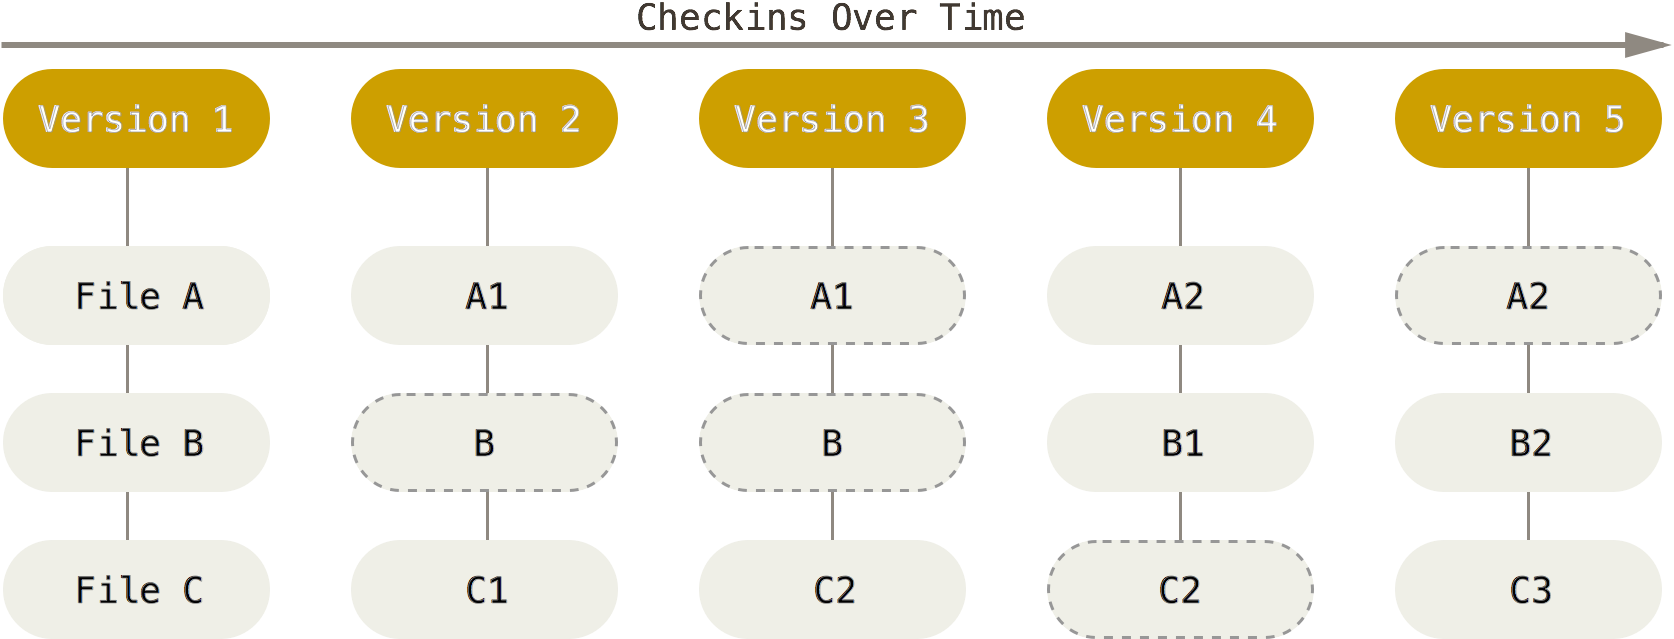
\includegraphics{images/snapshots}
  \caption{Git stocke les données comme des instantanés du projet au cours du temps}
  \label{fig:git:snapshots}
\end{figure}

C'est une distinction importante entre Git et quasiment tous les autres VCS.
Git a reconsidéré quasiment tous les aspects de la gestion de version que la plupart des autres systèmes ont copiés des générations précédentes.
Git ressemble beaucoup plus à un mini système de fichiers avec des outils incroyablement puissants construits dessus, plutôt qu'à un simple VCS.
Nous explorerons les bénéfices qu'il y a à penser les données de cette manière quand nous aborderons la gestion de branches dans la \autoref{sec:git:branching}.

\subsubsection{Presque toutes les opérations sont locales}

La plupart des opérations de Git ne nécessitent que des fichiers et ressources locaux  --- généralement aucune information venant d'un autre ordinateur du réseau n'est nécessaire.
Si vous êtes habitué à un CVCS où toutes les opérations sont ralenties par la latence des échanges réseau, cet aspect de Git vous fera penser que les dieux de la vitesse ont octroyé leurs pouvoirs à Git.
Comme vous disposez de l'historique complet du projet localement sur votre disque dur, la plupart des opérations semblent instantanées.

Par exemple, pour parcourir l'historique d'un projet, Git n'a pas besoin d'aller le chercher sur un serveur pour vous l'afficher ;
il n'a qu'à simplement le lire directement dans votre base de données locale.
Cela signifie que vous avez quasi-instantanément accès à l'historique du projet.
Si vous souhaitez connaître les modifications introduites entre la version actuelle d'un fichier et son état un mois auparavant, Git peut rechercher l'état du fichier un mois auparavant et réaliser le calcul de différence, au lieu d'avoir à demander cette différence à un serveur ou de devoir récupérer l'ancienne version sur le serveur pour calculer la différence localement.

Cela signifie aussi qu'il y a très peu de choses que vous ne puissiez réaliser si vous n'êtes pas connecté ou hors VPN.
Si vous voyagez en train ou en avion et voulez avancer votre travail, vous pouvez continuer à gérer vos versions sans soucis en attendant de pouvoir de nouveau vous connecter pour partager votre travail.
Si vous êtes chez vous et ne pouvez avoir une liaison VPN avec votre entreprise, vous pouvez tout de même travailler.
Pour de nombreux autres systèmes, faire de même est impossible ou au mieux très contraignant.
Avec Perforce par exemple, vous ne pouvez pas faire grand-chose tant que vous n'êtes pas connecté au serveur.
Avec Subversion ou CVS, vous pouvez éditer les fichiers, mais vous ne pourrez pas soumettre des modifications à votre base de données (car celle-ci est sur le serveur non accessible).
Cela peut sembler peu important a priori, mais vous seriez étonné de découvrir quelle grande différence cela peut constituer à l'usage.

\subsubsection{Git gère l'intégrité}

Dans Git, tout est vérifié par une somme de contrôle avant d'être stocké et par la suite cette somme de contrôle, signature unique, sert de référence.
Cela signifie qu'il est impossible de modifier le contenu d'un fichier ou d'un répertoire sans que Git ne s'en aperçoive.
Cette fonctionnalité est ancrée dans les fondations de Git et fait partie intégrante de sa philosophie.
Vous ne pouvez pas perdre des données en cours de transfert ou corrompre un fichier sans que Git ne puisse le détecter.

Le mécanisme que Git utilise pour réaliser les sommes de contrôle est appelé une empreinte SHA-1.
C'est une chaîne de caractères composée de 40 caractères hexadécimaux (de $0$ à $9$ et de «a» à «f») calculée en fonction du contenu du fichier ou de la structure du répertoire considéré.
Une empreinte SHA-1 ressemble à ceci :
\begin{Schunk}
\begin{Verbatim}
24b9da6552252987aa493b52f8696cd6d3b00373
\end{Verbatim}
\end{Schunk}

Vous trouverez ces valeurs à peu près partout dans Git car il les utilise pour tout.
En fait, Git stocke tout non pas avec des noms de fichiers, mais dans la base de données Git indexée par ces valeurs.

\subsubsection{Généralement, Git ne fait qu'ajouter des données}

Quand vous réalisez des actions dans Git, la quasi-totalité d'entre elles ne font qu'ajouter des données dans la base de données de Git.
Il est très difficile de faire réaliser au système des actions qui ne soient pas réversibles ou de lui faire effacer des données d'une quelconque manière.
Par contre, comme dans la plupart des systèmes de gestion de version, vous pouvez perdre ou corrompre des modifications qui n'ont pas encore été entrées en base ;
mais dès que vous avez validé un instantané dans Git, il est très difficile de le perdre, spécialement si en plus vous synchronisez votre base de données locale avec un dépôt distant.

Cela fait de l'usage de Git un vrai plaisir, car on peut expérimenter sans danger de casser définitivement son projet.
Pour une information plus approfondie sur la manière dont Git stocke ses données et comment récupérer des données qui pourraient sembler perdues, référez-vous à la \autoref{sec:git:undoing}.

\subsubsection{Les trois états}

Un peu de concentration maintenant.
Il est primordial de se souvenir de ce qui suit si vous souhaitez que le reste de votre apprentissage s'effectue sans difficulté.
Git gère trois états dans lesquels les fichiers peuvent résider : validé, modifié et indexé.
Validé signifie que les données sont stockées en sécurité dans votre base de données locale.
Modifié signifie que vous avez modifié le fichier mais qu'il n'a pas encore été validé en base.
Indexé signifie que vous avez marqué un fichier modifié dans sa version actuelle pour qu'il fasse partie du prochain instantané du projet.

Ceci nous mène aux trois sections principales d'un projet Git : le répertoire Git, le répertoire de travail et la zone d'index.

\begin{figure}[H]
  \centering
  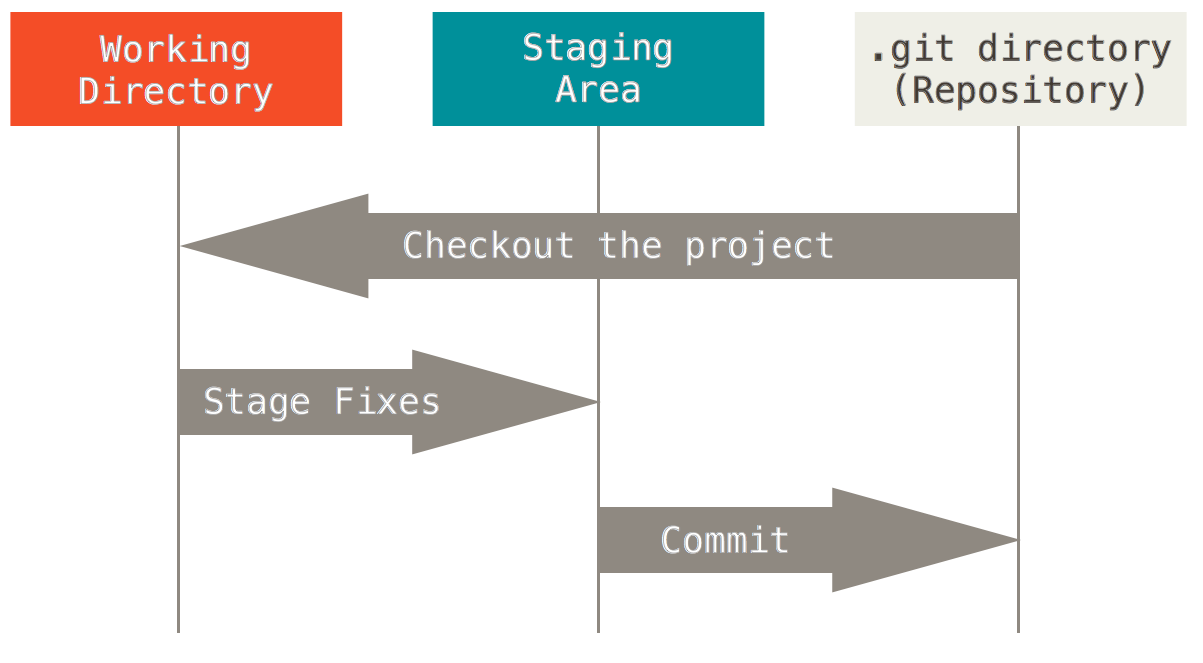
\includegraphics{images/areas}
  \caption{Répertoire de travail, zone d'index et répertoire Git}
  \label{fig:git:areas}
\end{figure}

Le répertoire Git est l'endroit où Git stocke les méta-données et la base de données des objets de votre projet.
C'est la partie la plus importante de Git, et c'est ce qui est copié lorsque vous clonez un dépôt depuis un autre ordinateur.

Le répertoire de travail est une extraction unique d'une version du projet.
Ces fichiers sont extraits depuis la base de données compressée dans le répertoire Git et placés sur le disque pour pouvoir être utilisés ou modifiés.

La zone d'index est un simple fichier, généralement situé dans le répertoire Git, qui stocke les informations concernant ce qui fera partie du prochain instantané. On l'appelle aussi des fois la zone de préparation.

L'utilisation standard de Git se passe comme suit :
\begin{enumerate}
\item vous modifiez des fichiers dans votre répertoire de travail ;
\item vous indexez les fichiers modifiés, ce qui ajoute des instantanés de ces fichiers dans la zone d'index ;
\item vous validez, ce qui a pour effet de basculer les instantanés des fichiers de l'index dans la base de données du répertoire Git.
\end{enumerate}

Si une version particulière d'un fichier est dans le répertoire Git, il est considéré comme validé.
S'il est modifié mais a été ajouté dans la zone d'index, il est indexé.
S'il a été modifié depuis le dernier instantané mais n'a pas été indexé, il est modifié.
Dans la \autoref{sec:git:basics}, vous en apprendrez plus sur ces états et comment vous pouvez en tirer parti ou complètement occulter la phase d'indexation.

\subsection{La ligne de commande}

Il existe de nombreuses manières différentes d'utiliser Git.
Il y a les outils originaux en ligne de commande et il y a de nombreuses interfaces graphiques avec des capacités variables.
Dans ce livre, nous utiliserons Git en ligne de commande.
Tout d'abord, la ligne de commande est la seule interface qui permet de lancer \emph{toutes} les commandes Git --- la plupart des interfaces graphiques simplifient l'utilisation en ne couvrant qu'un sous-ensemble des fonctionnalités de Git.
Si vous savez comment utiliser la version en ligne de commande, vous serez à même de comprendre comment fonctionne la version graphique, tandis que l'inverse n'est pas nécessairement vrai.
De plus, le choix d'un outil graphique est sujet à des goûts personnels, mais \emph{tous} les utilisateurs auront les commandes en lignes installées et utilisables.

Nous considérons que vous savez ouvrir un Terminal sous Mac ou une invite de commandes ou Powershell sous Windows.
Si ce n'est pas le cas, il va falloir tout d'abord vous renseigner sur ces applications pour pouvoir comprendre la suite des exemples et descriptions du livre.

\subsection{Paramétrage à la première utilisation de Git}
\label{sec:git:first_time}

Maintenant que vous avez installé Git sur votre système, vous voudrez personnaliser votre environnement Git.
Vous ne devriez avoir à réaliser ces réglages qu'une seule fois;
ils persisteront lors des mises à jour.
Vous pouvez aussi les changer à tout instant en relançant les mêmes commandes.

Git contient un outil appelé \code{git config} pour vous permettre de voir et modifier les variables de configuration qui contrôlent tous les aspects de l'apparence et du comportement de Git.
Ces variables peuvent être stockées dans trois endroits différents:
\begin{itemize}
\item Fichier \code{/etc/gitconfig}: Contient les valeurs pour tous les utilisateurs et tous les dépôts du système.
Si vous passez l'option \code{--system} à \code{git config}, il lit et écrit ce fichier spécifiquement.
\item Fichier \verb=~/.gitconfig=: Spécifique à votre utilisateur.
Vous pouvez forcer Git à lire et écrire ce fichier en passant l'option \code{--global}.
\item Fichier \code{config} dans le répertoire Git (c'est-à-dire \code{.git/config}) du dépôt en cours d'utilisation: spécifique au seul dépôt en cours.
\end{itemize}
Chaque niveau surcharge le niveau précédent, par conséquent les valeurs dans \code{.git/config} surchargent celles de \code{/etc/gitconfig}.

Sur les systèmes Windows, Git recherche le fichier \code{.gitconfig} dans le répertoire \code{\$HOME} (\code{\%USERPROFILE\%} dans l’environnement natif de Windows) qui est \code{C:{\bs}Users{\bs}\$USER} la plupart du temps, selon la version (\code{\$USER} devient \code{\%USERNAME\%} dans l’environnement de Windows).
Il recherche tout de même \code{/etc/gitconfig}, bien qu'il soit relatif à la racine MSys, qui se trouve où vous aurez décidé d'installer Git sur votre système Windows.
Si vous utilisez une version 2.x ou supérieure de Git pour Windows, il y a aussi un fichier de configuration système dans \code{C:{\bs}ProgramData{\bs}Git{\bs}config} sur Windows Vista et supérieur.
Ce fichier de configuration ne peut être modifié qu'avec la commande \code{git config -f \meta{fichier}} en tant qu'administrateur.

\subsubsection{Votre identité}

La première chose à faire après l'installation de Git est de renseigner votre nom et votre adresse de courriel.
C'est une information importante car toutes les validations dans Git utilisent cette information et elle est indélébile dans toutes les validations que vous pourrez réaliser:
\begin{Schunk}
\begin{Verbatim}
$ git config --global user.name "John Doe"
$ git config --global user.email johndoe@example.com
\end{Verbatim}
\end{Schunk}

Encore une fois, cette étape n'est nécessaire qu'une fois si vous passez l'option \code{--global}, parce que Git utilisera toujours cette information pour tout ce que votre utilisateur fera sur ce système.
Si vous souhaitez surcharger ces valeurs avec un nom ou une adresse de courriel différents pour un projet spécifique, vous pouvez lancer ces commandes sans option \code{--global} lorsque vous êtes dans ce projet.

De nombreux outils graphiques vous aideront à le faire la première fois que vous les lancerez.

\subsubsection{Votre éditeur de texte}

À présent que votre identité est renseignée, vous pouvez configurer l'éditeur de texte qui sera utilisé quand Git vous demande de saisir un message.
Par défaut, Git utilise l'éditeur configuré au niveau système, qui est généralement Vi ou Vim.
Si vous souhaitez utiliser un éditeur de texte différent, comme Emacs, vous pouvez entrer ce qui suit:
\begin{Schunk}
\begin{Verbatim}
$ git config --global core.editor emacs
\end{Verbatim}
\end{Schunk}

\warningbox{Vim et Emacs sont des éditeurs de texte populaires chez les développeurs sur les systèmes à base Unix tels que Linux et Mac.
Si vous n'êtes habitué à aucun de ces deux éditeurs ou utilisez un système Windows, il se peut que vous deviez chercher les instructions pour renseigner votre éditeur favori.
Si vous ne renseignez pas un éditeur et ne connaissez pas Vim ou Emacs, vous risquez fort d'avoir des surprises lorsqu'ils démarreront.}

\subsubsection{Vérifier vos paramètres}

Si vous souhaitez vérifier vos réglages, vous pouvez utiliser la commande \code{git config --list} pour lister tous les réglages que Git a pu trouver jusqu'ici:
\begin{Schunk}
\begin{Verbatim}
$ git config --list
user.name=John Doe
user.email=johndoe@example.com
color.status=auto
color.branch=auto
color.interactive=auto
color.diff=auto
...
\end{Verbatim}
\end{Schunk}

Vous pourrez voir certains paramètres apparaître plusieurs fois car Git lit les mêmes paramètres depuis plusieurs fichiers (par exemple \verb=~/.gitconfig= et \code{/etc/gitconfig}).
Git utilise la dernière valeur pour chaque paramètre.

Vous pouvez aussi vérifier la valeur effective d'un paramètre particulier en tapant \code{git config \meta{paramètre}}:
\begin{Schunk}
\begin{Verbatim}
$ git config user.name
John Doe
\end{Verbatim}
\end{Schunk}

\subsection{Obtenir de l'aide}
\label{sec:git:help}

Si vous avez besoin d'aide pour utiliser Git, il y a trois moyens d'obtenir les pages de manuel pour toutes les commandes de Git:

\begin{Schunk}
\begin{Verbatim}[commandchars=\\\{\}]
$ git help \meta{commande}
$ git \meta{commande} --help
$ man git-\meta{commande}
\end{Verbatim}
\end{Schunk}

Par exemple, vous pouvez obtenir la page de manuel pour la commande \code{config} en lançant:
\begin{Schunk}
\begin{Verbatim}
$ git help config
\end{Verbatim}
\end{Schunk}

Ces commandes sont vraiment sympathiques car vous pouvez y accéder depuis partout, y compris hors connexion.
Si les pages de manuel et ce livre ne sont pas suffisants, vous pouvez essayer les canaux \code{\#git} ou \code{\#github} sur le serveur IRC Freenode (\code{irc.freenode.net}).
Ces canaux sont régulièrement peuplés de centaines de personnes qui ont une bonne connaissance de Git et sont souvent prêtes à aider.

\subsection{Résumé}

Vous devriez avoir à présent une compréhension initiale de ce que Git est et en quoi il est différent des CVCS que vous pourriez déjà avoir utilisés.
Vous devriez aussi avoir une version de Git en état de fonctionnement sur votre système, paramétrée avec votre identité.
Il est temps d'apprendre les bases d'utilisation de Git.


\section{Les bases de Git}
\label{sec:git:basics}

Si vous ne deviez lire qu'un chapitre avant de commencer à utiliser Git, c'est celui-ci.
Ce chapitre couvre les commandes de base nécessaires pour réaliser la vaste majorité des activités avec Git.
À la fin de ce chapitre, vous devriez être capable de configurer et initialiser un dépôt, commencer et arrêter le suivi de version de fichiers, d'indexer et valider des modifications.
Nous vous montrerons aussi comment paramétrer Git pour qu'il ignore certains fichiers ou patrons de fichiers, comment revenir sur les erreurs rapidement et facilement, comment parcourir l'historique de votre projet et voir les modifications entre deux validations, et comment pousser et tirer les modifications avec des dépôts distants.

\subsection{Démarrer un dépôt Git}
\label{sec:git:getting_a_repo}

Vous pouvez principalement démarrer un dépôt Git de deux manières.
La première consiste à prendre un projet ou un répertoire existant et à l'importer dans Git.
La seconde consiste à cloner un dépôt Git existant sur un autre serveur.

\subsubsection{Initialisation d'un dépôt Git dans un répertoire existant}

Si vous commencez à suivre un projet existant dans Git, vous n'avez qu'à vous positionner dans le répertoire du projet et saisir:
\begin{Schunk}
\begin{Verbatim}
$ git init
\end{Verbatim}
\end{Schunk}

Cela crée un nouveau sous-répertoire nommé \code{.git} qui contient tous les fichiers nécessaires au dépôt --- un squelette de dépôt Git.
Pour l'instant, aucun fichier n'est encore versionné.
(consulter \emph{Les tripes de Git} pour plus d'information sur les fichiers contenus dans le répertoire \code{.git} que vous venez de créer.)
\begin{Schunk}
\begin{Verbatim}
$ git add *.c
$ git add LICENSE
$ git commit -m 'initial project version'
\end{Verbatim}
\end{Schunk}

\subsubsection{Cloner un dépôt existant}
\label{sec:git:cloning}

Si vous souhaitez obtenir une copie d'un dépôt Git existant --- par exemple, un projet auquel vous aimeriez contribuer --- la commande dont vous avez besoin s'appelle \code{git clone}.
Si vous êtes familier avec d'autres systèmes de gestion de version tels que Subversion, vous noterez que la commande est \code{clone} et non \code{checkout}.
C'est une distinction importante --- Git reçoit une copie de quasiment toutes les données dont le serveur dispose.
Toutes les versions de tous les fichiers pour l'historique du projet sont téléchargées quand vous lancez \code{git clone}.
En fait, si le disque du serveur se corrompt, vous pouvez utiliser n'importe quel clone pour remettre le serveur dans l'état où il était au moment du clonage (vous pourriez perdre quelques paramètres du serveur, mais toutes les données sous gestion de version seraient récupérées --- consulter \emph{Installation de Git sur un serveur} pour de plus amples détails).

Vous clonez un dépôt avec \code{git clone \meta{url}}.
Par exemple, si vous voulez cloner la bibliothèque logicielle Git appelée libgit2, vous pouvez le faire de la manière suivante:
\begin{Schunk}
\begin{Verbatim}
$ git clone https://github.com/libgit2/libgit2
\end{Verbatim}
\end{Schunk}

Ceci crée un répertoire nommé \code{libgit2}, initialise un répertoire \code{.git} à l'intérieur, récupère toutes les données de ce dépôt, et extrait une copie de travail de la dernière version.
Si vous examinez le nouveau répertoire \code{libgit2}, vous y verrez les fichiers du projet, prêts à être modifiés ou utilisés.
Si vous souhaitez cloner le dépôt dans un répertoire nommé différemment, vous pouvez spécifier le nom dans une option supplémentaire de la ligne de commande:
\begin{Schunk}
\begin{Verbatim}
$ git clone https://github.com/libgit2/libgit2 monlibgit2
\end{Verbatim}
\end{Schunk}

Cette commande réalise la même chose que la précédente, mais le répertoire cible s'appelle \code{monlibgit2}.

Git dispose de différents protocoles de transfert que vous pouvez utiliser.
L'exemple précédent utilise le protocole \code{https://}, mais vous pouvez aussi voir \code{git://} ou \code{utilisateur@serveur:/chemin.git}, qui utilise le protocole de transfert SSH.
\emph{Installation de Git sur un serveur} introduit toutes les options disponibles pour mettre en place un serveur Git, ainsi que leurs avantages et inconvénients.

\subsection{Enregistrer des modifications dans le dépôt}

Vous avez à présent un dépôt Git valide et une extraction ou copie de travail du projet.
Vous devez faire quelques modifications et valider des instantanés de ces modifications dans votre dépôt chaque fois que votre projet atteint un état que vous souhaitez enregistrer.

Souvenez-vous que chaque fichier de votre copie de travail peut avoir deux états: sous suivi de version ou non suivi.
Les fichiers suivis sont les fichiers qui appartenaient déjà au dernier instantané; ils peuvent être inchangés, modifiés ou indexés.
Tous les autres fichiers sont non suivis --- tout fichier de votre copie de travail qui n'appartenait pas à votre dernier instantané et n'a pas été indexé.
Quand vous clonez un dépôt pour la première fois, tous les fichiers seront sous suivi de version et inchangés car Git vient tout juste de les extraire et vous ne les avez pas encore édités.

Au fur et à mesure que vous éditez des fichiers, Git les considère comme modifiés, car vous les avez modifiés depuis le dernier instantané.
Vous \emph{indexez} ces fichiers modifiés et vous enregistrez toutes les modifications indexées, puis ce cycle se répète.

\begin{figure}[H]
  \centering
  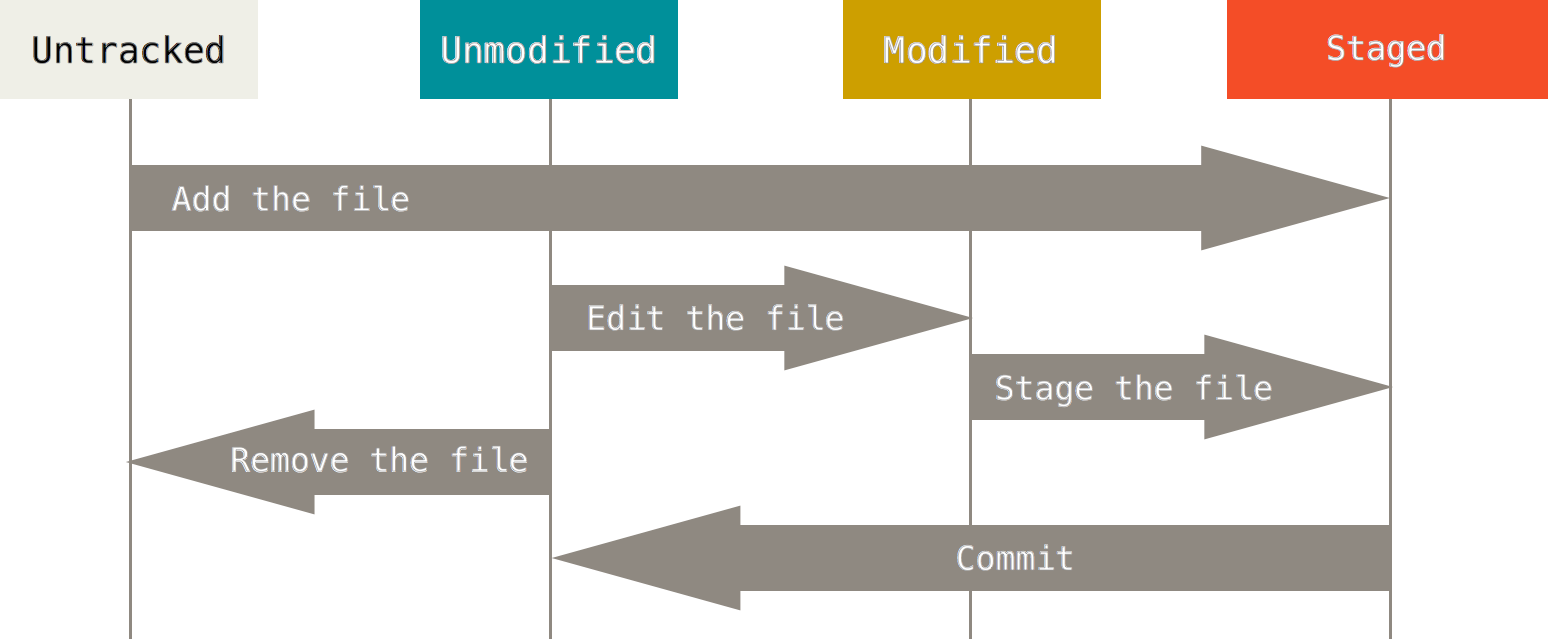
\includegraphics{images/lifecycle}
  \caption{Le cycle de vie des états des fichiers}
  \label{fig:git:lifecycle}
\end{figure}

\subsubsection{Vérifier l'état des fichiers}
\label{sec:git:checking_status}

L'outil principal pour déterminer quels fichiers sont dans quel état est la commande \code{git status}.
Si vous lancez cette commande juste après un clonage, vous devriez voir ce qui suit:
\begin{Schunk}
\begin{Verbatim}
$ git status
Sur la branche master
Votre branche est à jour avec 'origin/master'.
rien à valider, la copie de travail est propre
\end{Verbatim}
\end{Schunk}

Ce message signifie que votre copie de travail est propre,en d'autres termes, aucun fichier suivi n'a été modifié.
Git ne voit pas non plus de fichiers non-suivis, sinon ils seraient listés ici.
Enfin, la commande vous indique sur quelle branche vous êtes.
Pour l'instant, c'est toujours \code{master}, qui correspond à la valeur par défaut; nous ne nous en soucierons pas maintenant.
Dans la \autoref{sec:git:branching}, nous parlerons plus en détail des branches et des références.

Supposons que vous souhaitez ajouter un nouveau fichier au projet, un simple fichier \code{LISEZMOI}.
Si le fichier n'existait pas auparavant, et si vous lancez \code{git status}, vous voyez votre fichier non suivi comme suit:
\begin{Schunk}
\begin{Verbatim}
$ echo 'Mon Projet' > LISEZMOI
$ git status
Sur la branche master
Votre branche est à jour avec 'origin/master'.
Fichiers non suivis:
  (utilisez "git add <fichier>..." pour inclure dans ce
   qui sera validé)

        LISEZMOI

aucune modification ajoutée à la validation mais des
fichiers non suivis sont présents (utilisez "git add" pour
les suivre)
\end{Verbatim}
\end{Schunk}

Vous pouvez constater que votre nouveau fichier \code{LISEZMOI} n'est pas en suivi de version, car il apparaît dans la section «Fichiers non suivis» de l'état de la copie de travail.
«non suivi» signifie simplement que Git détecte un fichier qui n'était pas présent dans le dernier instantané; Git ne le placera sous suivi de version que quand vous lui indiquerez de le faire.
Ce comportement permet de ne pas placer accidentellement sous suivi de version des fichiers binaires générés ou d'autres fichiers que vous ne voulez pas inclure.
Mais vous voulez inclure le fichier \code{LISEZMOI} dans l'instantané, alors commençons à suivre ce fichier.

\subsubsection{Placer de nouveaux fichiers sous suivi de version}
\label{sec:git:tracking_files}

Pour commencer à suivre un nouveau fichier, vous utilisez la commande \code{git add}.
Pour commencer à suivre le fichier \code{LISEZMOI}, vous pouvez entrer ceci:
\begin{Schunk}
\begin{Verbatim}
$ git add LISEZMOI
\end{Verbatim}
\end{Schunk}

Si vous lancez à nouveau la commande \code{git status}, vous pouvez constater que votre fichier \code{LISEZMOI} est maintenant suivi et indexé:
\begin{Schunk}
\begin{Verbatim}
$ git status
Sur la branche master
Votre branche est à jour avec 'origin/master'.
Modifications qui seront validées :
  (utilisez "git reset HEAD <fichier>..." pour désindexer)

        nouveau fichier: LISEZMOI
\end{Verbatim}
\end{Schunk}

Vous pouvez affirmer qu'il est indexé car il apparaît dans la section «Modifications qui seront validées».
Si vous validez à ce moment, la version du fichier à l'instant où vous lancez \code{git add} est celle qui sera dans l'historique des instantanés.
Vous pouvez vous souvenir que lorsque vous avez précédemment lancé \code{git init}, vous avez ensuite lancé \code{git add \meta{fichiers}} --- c'était bien sûr pour commencer à placer sous suivi de version les fichiers de votre répertoire de travail.
La commande \code{git add} accepte en paramètre un chemin qui correspond à un fichier ou un répertoire; dans le cas d'un répertoire, la commande ajoute récursivement tous les fichiers de ce répertoire.

\subsubsection{Indexer des fichiers modifiés}

Maintenant, modifions un fichier qui est déjà sous suivi de version.
Si vous modifiez le fichier sous suivi de version appelé \code{CONTRIBUTING.md} et que vous lancez à nouveau votre commande \code{git status}, vous verrez ceci:
\begin{Schunk}
\begin{Verbatim}
$ git status
Sur la branche master
Votre branche est à jour avec 'origin/master'.
Modifications qui seront validées :
  (utilisez "git reset HEAD <fichier>..." pour désindexer)

        nouveau fichier: LISEZMOI

Modifications qui ne seront pas validées :
  (utilisez "git add <fichier>..." pour mettre à jour ce
   qui sera validé)
  (utilisez "git checkout -- <fichier>..." pour annuler les
   modifications dans la copie de travail)

        modifié:         CONTRIBUTING.md
\end{Verbatim}
\end{Schunk}

Le fichier \code{CONTRIBUTING.md} apparaît sous la section nommée «Modifications qui ne seront pas validées» ce qui signifie que le fichier sous suivi de version a été modifié dans la copie de travail mais n'est pas encore indexé.
Pour l'indexer, il faut lancer la commande \code{git add}. \code{git add} est une commande multi-usage --- elle peut être utilisée pour placer un fichier sous suivi de version, pour indexer un fichier ou pour d'autres actions telles que marquer comme résolus des conflits de fusion de fichiers.
Sa signification s'approche plus de «ajouter ce contenu pour la prochaine validation» que de «ajouter ce contenu au projet».
Lançons maintenant \code{git add} pour indexer le fichier \code{CONTRIBUTING.md}, et relançons la commande \code{git status}:
\begin{Schunk}
\begin{Verbatim}
$ git status
Sur la branche master
Votre branche est à jour avec 'origin/master'.
Modifications qui seront validées :
  (utilisez "git reset HEAD <fichier>..." pour désindexer)

        nouveau fichier: LISEZMOI
        modifié:         CONTRIBUTING.md

\end{Verbatim}
\end{Schunk}

À présent, les deux fichiers sont indexés et feront partie de la prochaine validation.
Mais supposons que vous souhaitiez apporter encore une petite modification au fichier \code{CONTRIBUTING.md} avant de réellement valider la nouvelle version.
Vous l'ouvrez à nouveau, réalisez la petite modification et vous voilà prêt à valider.
Néanmoins, vous lancez \code{git status} une dernière fois:
\begin{Schunk}
\begin{Verbatim}
$ vim CONTRIBUTING.md
$ git status
Sur la branche master
Votre branche est à jour avec 'origin/master'.
Modifications qui seront validées :
  (utilisez "git reset HEAD <fichier>..." pour désindexer)

        nouveau fichier: LISEZMOI
        modifié:         CONTRIBUTING.md

Modifications qui ne seront pas validées :
  (utilisez "git add <fichier>..." pour mettre à jour ce
   qui sera validé)
  (utilisez "git checkout -- <fichier>..." pour annuler les
   modifications dans la copie de travail)

        modifié:         CONTRIBUTING.md
\end{Verbatim}
\end{Schunk}

Que s'est-il donc passé?
À présent, \code{CONTRIBUTING.md} apparaît à la fois comme indexé et non indexé.
En fait, Git indexe un fichier dans son état au moment où la commande \code{git add} est lancée.
Si on valide les modifications maintenant, la version de \code{CONTRIBUTING.md} qui fera partie de l'instantané est celle correspondant au moment où a été lancée la commande \code{git add CONTRIBUTING.md}, et non la version actuellement présente dans la copie de travail au moment où la commande \code{git commit} est lancée.
Si le fichier est modifié après un \code{git add}, il faut relancer \code{git add} pour prendre en compte l'état actuel de la copie de travail:
\begin{Schunk}
\begin{Verbatim}
$ git add CONTRIBUTING.md
$ git status
Sur la branche master
Votre branche est à jour avec 'origin/master'.
Modifications qui seront validées :
  (utilisez "git reset HEAD <fichier>..." pour désindexer)

        nouveau fichier: LISEZMOI
        modifié:         CONTRIBUTING.md

\end{Verbatim}
\end{Schunk}

\subsubsection{Statut court}

Bien que \code{git status} soit informatif, il est aussi plutôt verbeux.
Git a aussi une option de status court qui permet de voir les modifications de façon plus compacte.
Si vous lancez \code{git status -s} ou \code{git status --short}, vous obtenez une information bien plus simple.

\begin{Schunk}
\begin{Verbatim}
$ git status -s
 M README
MM Rakefile
A  lib/git.rb
M  lib/simplegit.rb
?? LICENSE.txt
\end{Verbatim}
\end{Schunk}

Les nouveaux fichiers qui ne sont pas suivis sont précédés de \code{??}, les fichiers nouveaux et indexés sont précédés de \code{A}, les fichiers modifiés de \code{M} et ainsi de suite.
Il y a deux colonnes d'état --- celle de gauche indique l'état de l'index et celle de droite l'état du dossier de travail.
Donc l'exemple ci-dessus indique que le fichier \code{README} est modifié dans le répertoire de travail mais n'est pas encore indexé, tandis que le fichier \code{lib/simplegit.rb} est modifié et indexé.
Le fichier \code{Rakefile} a été modifié, indexé puis modifié à nouveau, de sorte qu'il a des modifications à la fois indexées et non-indexées.

\subsubsection{Ignorer des fichiers}
\label{sec:git:ignoring}

Il apparaît souvent qu'un type de fichiers présent dans la copie de travail ne doit pas être ajouté automatiquement ou même ne doit pas apparaître comme fichier potentiel pour le suivi de version.
Ce sont par exemple des fichiers générés automatiquement tels que les fichiers de journaux ou de sauvegardes produits par l'outil que vous utilisez.
Dans un tel cas, on peut énumérer les patrons de noms de fichiers à ignorer dans un fichier \code{.gitignore}.
Voici ci-dessous un exemple de fichier \code{.gitignore}:
\begin{Schunk}
\begin{Verbatim}
$ cat .gitignore
*.[oa]
*~
\end{Verbatim}
\end{Schunk}

La première ligne ordonne à Git d'ignorer tout fichier se terminant en \code{.o} ou \code{.a} --- des fichiers objet ou archive qui sont généralement produits par la compilation d'un programme.
La seconde ligne indique à Git d'ignorer tous les fichiers se terminant par un tilde (\verb=~=), ce qui est le cas des noms des fichiers temporaires pour de nombreux éditeurs de texte tels que Emacs.
On peut aussi inclure un répertoire \code{log}, \code{tmp} ou \code{pid}, ou le répertoire de documentation générée automatiquement, ou tout autre fichier.
Renseigner un fichier \code{.gitignore} avant de commencer à travailler est généralement une bonne idée qui évitera de valider par inadvertance des fichiers qui ne doivent pas apparaître dans le dépôt Git.

Les règles de construction des patrons à placer dans \code{.gitignore} sont les suivantes:
\begin{itemize}
\item les lignes vides ou commençant par \code{\#} sont ignorées;
\item les patrons standards de fichiers sont utilisables;
\item si le patron se termine par une barre oblique (\code{/}), il indique un répertoire;
\item un patron commençant par un point d'exclamation (\code{!}) indique des fichiers à inclure malgré les autres règles
\end{itemize}

Les patrons standards de fichiers sont des expressions régulières simplifiées utilisées par les shells.
Un astérisque (\code{*}) correspond à un ou plusieurs caractères; \code{[abc]} correspond à un des trois caractères listés dans les crochets, donc a ou b ou c; un point d'interrogation (\code{?}) correspond à un unique caractère; des crochets entourant des caractères séparés par un tiret (\code{[0-9]}) correspond à un caractère dans l'intervalle des deux caractères indiqués, donc ici de 0 à 9.
Vous pouvez aussi utiliser deux astérisques pour indiquer une série de répertoires inclus; \code{a/**/z} correspond donc à \code{a/z}, \code{a/b/z}, \code{a/b/c/z} et ainsi de suite.

Voici un autre exemple de fichier \code{.gitignore}:
\begin{Schunk}
\begin{Verbatim}
# pas de fichier .a
*.a

# mais suivre lib.a malgré la règle précédente
!lib.a

# ignorer uniquement le fichier TODO à la racine du projet
/TODO

# ignorer tous les fichiers dans le répertoire build
build/

# ignorer doc/notes.txt, mais pas doc/server/arch.txt
doc/*.txt

# ignorer tous les fichiers .txt sous le répertoire doc/
doc/**/*.txt
\end{Verbatim}
\end{Schunk}

\tipbox{GitHub maintient une liste assez complète d'exemples de
  fichiers \code{.gitignore} correspondant à de nombreux types de
  projets et langages. Voir
  \link{https://github.com/github/gitignore}{} pour obtenir un point
  de départ pour votre projet.}

\subsubsection{Inspecter les modifications indexées et non indexées}
\label{sec:git:diff_staged}

Si le résultat de la commande \code{git status} est encore trop vague --- lorsqu'on désire savoir non seulement quels fichiers ont changé mais aussi ce qui a changé dans ces fichiers --- on peut utiliser la commande \code{git diff}.
Cette commande sera traitée en détail plus loin; mais elle sera vraisemblablement utilisée le plus souvent pour répondre aux questions suivantes: qu'est-ce qui a été modifié mais pas encore indexé? Quelle modification a été indexée et est prête pour la validation? Là où \code{git status} répond de manière générale à ces questions, \code{git diff} montre les lignes exactes qui ont été ajoutées, modifiées ou effacées --- le patch en somme.
\begin{Schunk}
\begin{Verbatim}
$ git status
Sur la branche master
Votre branche est à jour avec 'origin/master'.
Modifications qui seront validées :
  (utilisez "git reset HEAD <fichier>..." pour désindexer)

        nouveau fichier: LISEZMOI

Modifications qui ne seront pas validées :
  (utilisez "git add <fichier>..." pour mettre à jour ce
   qui sera validé)
  (utilisez "git checkout -- <fichier>..." pour annuler les
   modifications dans la copie de travail)

        modifié:         CONTRIBUTING.md
\end{Verbatim}
\end{Schunk}

Pour visualiser ce qui a été modifié mais pas encore indexé, tapez \code{git diff} sans autre argument:
\begin{Schunk}
\begin{Verbatim}[commandchars=\\\{\}]
$ git diff
diff --git a/CONTRIBUTING.md b/CONTRIBUTING.md
index 8ebb991..643e24f 100644
--- a/CONTRIBUTING.md
+++ b/CONTRIBUTING.md
@@ -65,7 +65,8 @@ branch directly, things can get messy.
 Please include a nice description of your changes whe\meta{...}
 if we have to read the whole diff to figure out why y\meta{...}
 in the first place, you're less likely to get feedbac\meta{...}
-merged in.
+merged in. Also, split your changes into comprehensiv\meta{...}
+longer than a dozen lines.

 If you are starting to work on a particular area, feel\meta{...}
 that highlights your work in progress (and note in the\meta{...}
\end{Verbatim}
\end{Schunk}

Cette commande compare le contenu du répertoire de travail avec la zone d'index.
Le résultat vous indique les modifications réalisées mais non indexées.

Si vous souhaitez visualiser les modifications indexées qui feront partie de la prochaine validation, vous pouvez utiliser \code{git diff --cached} (avec les versions 1.6.1 et supérieures de Git, vous pouvez aussi utiliser \code{git diff --staged}, qui est plus mnémotechnique).
Cette commande compare les fichiers indexés et le dernier instantané:
\begin{Schunk}
\begin{Verbatim}
$ git diff --staged
diff --git a/LISEZMOI b/LISEZMOI
new file mode 100644
index 0000000..1e17b0c
--- /dev/null
+++ b/LISEZMOI
@@ -0,0 +1 @@
+Mon Projet
\end{Verbatim}
\end{Schunk}

Il est important de noter que \code{git diff} ne montre pas les modifications réalisées depuis la dernière validation --- seulement les modifications qui sont non indexées.
Cela peut introduire une confusion car si tous les fichiers modifiés ont été indexés, \code{git diff} n'indiquera aucun changement.

Par exemple, si vous indexez le fichier \code{CONTRIBUTING.md} et l'éditez ensuite, vous pouvez utiliser \code{git diff} pour visualiser les modifications indexées et non indexées de ce fichier. Si l'état est le suivant:
\begin{Schunk}
\begin{Verbatim}
$ git add CONTRIBUTING.md
$ echo 'ligne de test' >> CONTRIBUTING.md
$ git status
Sur la branche master
Votre branche est à jour avec 'origin/master'.
Modifications qui seront validées :
  (utilisez "git reset HEAD <fichier>..." pour désindexer)

        nouveau fichier: CONTRIBUTING.md

Modifications qui ne seront pas validées :
  (utilisez "git add <fichier>..." pour mettre à jour ce
   qui sera validé)
  (utilisez "git checkout -- <fichier>..." pour annuler les
   modifications dans la copie de travail)

        modifié:         CONTRIBUTING.md
\end{Verbatim}
\end{Schunk}

À présent, vous pouvez utiliser \code{git diff} pour visualiser les modifications non indexées:
\begin{Schunk}
\begin{Verbatim}[commandchars=\\\{\}]
$ git diff
diff --git a/CONTRIBUTING.md b/CONTRIBUTING.md
index 643e24f..87f08c8 100644
--- a/CONTRIBUTING.md
+++ b/CONTRIBUTING.md
@@ -119,3 +119,4 @@ at the
 ## Starter Projects

 See our [projects list](https://github.com/libgit2/lib\meta{...}
+ligne de test
\end{Verbatim}
\end{Schunk}

La commande \code{git diff --cached} permet de visualiser ce qui a été indexé jusqu'à maintenant:
\begin{Schunk}
\begin{Verbatim}[commandchars=\\\{\}]
$ git diff --cached
diff --git a/CONTRIBUTING.md b/CONTRIBUTING.md
index 8ebb991..643e24f 100644
--- a/CONTRIBUTING.md
+++ b/CONTRIBUTING.md
@@ -65,7 +65,8 @@ branch directly, things can get messy.
 Please include a nice description of your changes when\meta{...}
 if we have to read the whole diff to figure out why yo\meta{...}
 in the first place, you're less likely to get feedback\meta{...}
-merged in.
+merged in. Also, split your changes into comprehensive\meta{...}
+longer than a dozen lines.

 If you are starting to work on a particular area, feel\meta{...}
 that highlights your work in progress (and note in the\meta{...}
\end{Verbatim}
\end{Schunk}


\subsubsection{Valider vos modifications}
\label{sec:git:committing_changes}

Maintenant que votre zone d'index est dans l'état désiré, vous pouvez valider vos modifications.
Souvenez-vous que tout ce qui est encore non indexé --- tous les fichiers qui ont été créés ou modifiés mais n'ont pas subi de \code{git add} depuis que vous les avez modifiés  --- ne feront pas partie de la prochaine validation.
Ils resteront en tant que fichiers modifiés sur votre disque.

Dans notre cas, la dernière fois que vous avez lancé \code{git status}, vous avez vérifié que tout était indexé, et vous êtes donc prêt à valider vos modifications.
La manière la plus simple de valider est de taper \code{git commit}:
\begin{Schunk}
\begin{Verbatim}
$ git commit
\end{Verbatim}
\end{Schunk}

Cette action lance votre éditeur par défaut (qui est paramétré par la variable d'environnement \code{\$EDITOR} de votre shell --- habituellement vim ou Emacs, mais vous pouvez le paramétrer spécifiquement pour Git en utilisant la commande \code{git config --global core.editor} comme nous l'avons vu à la \autoref{sec:git:getting_started}).

L'éditeur affiche le texte suivant:
\begin{Schunk}
\begin{Verbatim}


# Veuillez saisir le message de validation pour vos
# modifications. Les lignes commençant par '#' seront
# ignorées, et un message vide abandonne la validation.
# Sur la branche master
# Votre branche est à jour avec 'origin/master'.
#
# Modifications qui seront validées :
#       nouveau fichier: LISEZMOI
#       modifié :         CONTRIBUTING.md
#
\end{Verbatim}
\end{Schunk}

Vous constatez que le message de validation par défaut contient une ligne vide suivie en commentaire par le résultat de \code{git status}.
Vous pouvez effacer ces lignes de commentaire et saisir votre propre message de validation, ou vous pouvez les laisser en place pour vous aider à vous rappeler ce que vous êtes en train de valider (pour un rappel plus explicite de ce que vous avez modifié, vous pouvez aussi passer l'option \code{-v} à la commande \code{git commit}.
Cette option place le résultat du diff en commentaire dans l'éditeur pour vous permettre de visualiser exactement ce que vous avez modifié.
Quand vous quittez l'éditeur (après avoir sauvegardé le message), Git crée votre \emph{commit} avec ce message de validation (après avoir retiré les commentaires et le diff).

Autrement, vous pouvez spécifier votre message de validation en ligne avec la commande \code{git commit} en le saisissant après l'option \code{-m}, comme ceci:
\begin{Schunk}
\begin{Verbatim}
$ git commit -m "Story 182: Fix benchmarks for speed"
[master 463dc4f] Story 182: Fix benchmarks for speed
 2 files changed, 2 insertions(+)
 create mode 100644 LISEZMOI
\end{Verbatim}
\end{Schunk}

À présent, vous avez créé votre premier \emph{commit}! Vous pouvez constater que le \emph{commit} vous fournit quelques informations sur lui-même: sur quelle branche vous avez validé (\code{master}), quelle est sa somme de contrôle SHA-1 (\code{463dc4f}), combien de fichiers ont été modifiés, et quelques statistiques sur les lignes ajoutées et effacées dans ce \emph{commit}.

Souvenez-vous que la validation enregistre l'instantané que vous avez préparé dans la zone d'index.
Tout ce que vous n'avez pas indexé est toujours en état modifié; vous pouvez réaliser une nouvelle validation pour l'ajouter à l'historique.
À chaque validation, vous enregistrez un instantané du projet en forme de jalon auquel vous pourrez revenir ou avec lequel comparer votre travail ultérieur.

\subsubsection{Passer l'étape de mise en index}

Bien qu'il soit incroyablement utile de pouvoir organiser les \emph{commits} exactement comme on l'entend, la gestion de la zone d'index est parfois plus complexe que nécessaire dans le cadre d'une utilisation normale.
Si vous souhaitez éviter la phase de placement des fichiers dans la zone d'index, Git fournit un raccourci très simple.
L'ajout de l'option \code{-a} à la commande \code{git commit} ordonne à Git de placer automatiquement tout fichier déjà en suivi de version dans la zone d'index avant de réaliser la validation, évitant ainsi d'avoir à taper les commandes \code{git add}:
\begin{Schunk}
\begin{Verbatim}
$ git status
Sur la branche master
Votre branche est à jour avec 'origin/master'.
Modifications qui ne seront pas validées :
  (utilisez "git add <fichier>..." pour mettre à jour ce
   qui sera validé)
  (utilisez "git checkout -- <fichier>..." pour annuler les
   modifications dans la copie de travail)

        modifié:         CONTRIBUTING.md

aucune modification n'a été ajoutée à la validation
(utilisez "git add" ou "git commit -a")
$ git commit -a -m 'added new benchmarks'
[master 83e38c7] added new benchmarks
 1 file changed, 5 insertions(+), 0 deletions(-)
\end{Verbatim}
\end{Schunk}

Notez que vous n'avez pas eu à lancer \code{git add} sur \code{CONTRIBUTING.md} avant de valider.

\subsubsection{Effacer des fichiers}
\label{sec:git:removing_files}

Pour effacer un fichier de Git, vous devez l'éliminer des fichiers en suivi de version (plus précisément, l'effacer dans la zone d'index) puis valider.
La commande \code{git rm} réalise cette action mais efface aussi ce fichier de votre copie de travail de telle sorte que vous ne le verrez pas réapparaître comme fichier non suivi en version à la prochaine validation.

Si vous effacez simplement le fichier dans votre copie de travail, il apparaît sous la section «Modifications qui ne seront pas validées» (c'est-à-dire, \emph{non indexé}) dans le résultat de \code{git status}:
\begin{Schunk}
\begin{Verbatim}
$ rm PROJECTS.md
$ git status
Sur la branche master
Votre branche est à jour avec 'origin/master'.
Modifications qui ne seront pas validées :
  (utilisez "git add/rm <fichier>..." pour mettre à jour ce
   qui sera validé)
  (utilisez "git checkout -- <fichier>..." pour annuler les
   modifications dans la copie de travail)

        supprimé:        PROJECTS.md

aucune modification n'a été ajoutée à la validation
(utilisez "git add" ou "git commit -a")
\end{Verbatim}
\end{Schunk}

Ensuite, si vous lancez \code{git rm}, l'effacement du fichier est indexé:
\begin{Schunk}
\begin{Verbatim}
$ git rm PROJECTS.md
rm 'PROJECTS.md'
Sur la branche master
Votre branche est à jour avec 'origin/master'.
Modifications qui seront validées :
  (utilisez "git reset HEAD <fichier>..." pour désindexer)

        supprimé:        PROJECTS.md
\end{Verbatim}
\end{Schunk}

Lors de la prochaine validation, le fichier sera absent et non-suivi en version.
Si vous avez auparavant modifié et indexé le fichier, son élimination doit être forcée avec l'option \code{-f}.
C'est une mesure de sécurité pour empêcher un effacement accidentel de données qui n'ont pas encore été enregistrées dans un instantané et qui seraient définitivement perdues.

Un autre scénario serait de vouloir abandonner le suivi de version d'un fichier tout en le conservant dans la copie de travail.
Ceci est particulièrement utile lorsqu'on a oublié de spécifier un patron dans le fichier \code{.gitignore} et on a accidentellement indexé un fichier, tel qu'un gros fichier de journal ou une série d'archives de compilation \code{.a}.
Pour réaliser ce scénario, utilisez l'option \code{--cached}:
\begin{Schunk}
\begin{Verbatim}
$ git rm --cached LISEZMOI
\end{Verbatim}
\end{Schunk}

Vous pouvez spécifier des noms de fichiers ou de répertoires, ou des patrons de fichiers à la commande \code{git rm}.
Cela signifie que vous pouvez lancer des commandes telles que:
\begin{Schunk}
\begin{Verbatim}
$ git rm log/\*.log
\end{Verbatim}
\end{Schunk}

Notez bien la barre oblique inverse (\code{\bs}) devant \code{*}.
Il est nécessaire d'échapper le caractère \code{*} car Git utilise sa propre expansion de nom de fichier en addition de l'expansion du shell. Ce caractère d'échappement doit être omis sous Windows si vous utilisez le terminal système.
Cette commande efface tous les fichiers avec l'extension \code{.log} présents dans le répertoire \code{log/}.
Vous pouvez aussi lancer une commande telle que:
\begin{Schunk}
\begin{Verbatim}
$ git rm \*~
\end{Verbatim}
\end{Schunk}

Cette commande élimine tous les fichiers se terminant par \verb=~=.

\subsubsection{Déplacer des fichiers}
\label{sec:git:mv}

À la différence des autres VCS, Git ne suit pas explicitement les mouvements des fichiers.
Si vous renommez un fichier suivi par Git, aucune méta-donnée indiquant le renommage n'est stockée par Git.
Néanmoins, Git est assez malin pour s'en apercevoir après coup --- la détection de mouvement de fichier sera traitée plus loin.

De ce fait, que Git ait une commande \code{mv} peut paraître trompeur.
Si vous souhaitez renommer un fichier dans Git, vous pouvez lancer quelque chose comme:
\begin{Schunk}
\begin{Verbatim}[commandchars=\\\{\}]
$ git mv \meta{nom\_origine} \meta{nom\_cible}
\end{Verbatim}
\end{Schunk}
et cela fonctionne.
En fait, si vous lancez quelque chose comme ceci et inspectez le résultat d'une commande \code{git status}, vous constaterez que Git gère le renommage de fichier:
\begin{Schunk}
\begin{Verbatim}
$ git mv LISEZMOI.txt LISEZMOI
$ git status
Sur la branche master
Votre branche est à jour avec 'origin/master'.
Modifications qui seront validées :
  (utilisez "git reset HEAD <fichier>..." pour désindexer)

        renommé:         LISEZMOI.txt -> LISEZMOI
\end{Verbatim}
\end{Schunk}

Néanmoins, cela revient à lancer les commandes suivantes:
\begin{Schunk}
\begin{Verbatim}
$ mv LISEZMOI.txt LISEZMOI
$ git rm LISEZMOI.txt
$ git add LISEZMOI
\end{Verbatim}
\end{Schunk}

Git trouve implicitement que c'est un renommage, donc cela importe peu si vous renommez un fichier de cette manière ou avec la commande \code{mv}.
La seule différence réelle est que \code{git mv} ne fait qu'une commande à taper au lieu de trois --- c'est une commande de convenance.
Le point principal est que vous pouvez utiliser n'importe quel outil pour renommer un fichier, et traiter les commandes \code{add}/\code{rm} plus tard, avant de valider la modification.

\subsection{Visualiser l'historique des validations}
\label{sec:git:viewing_history}

Après avoir créé plusieurs \emph{commits} ou si vous avez cloné un dépôt ayant un historique de \emph{commits}, vous souhaitez probablement revoir le fil des évènements.
Pour ce faire, la commande \code{git log} est l'outil le plus basique et le plus puissant.

Les exemples qui suivent utilisent le projet très simple \code{simplegit} conçu pour les démonstrations.
Pour récupérer le projet, lancez:
\begin{Schunk}
\begin{Verbatim}
git clone https://github.com/schacon/simplegit-progit
\end{Verbatim}
\end{Schunk}

Lorsque vous lancez \code{git log} dans le répertoire de ce projet, vous devriez obtenir un résultat qui ressemble à ceci:
\begin{Schunk}
\begin{Verbatim}
$ git log
commit ca82a6dff817ec66f44342007202690a93763949
Author: Scott Chacon <schacon@gee-mail.com>
Date:   Mon Mar 17 21:52:11 2008 -0700

    changed the version number

commit 085bb3bcb608e1e8451d4b2432f8ecbe6306e7e7
Author: Scott Chacon <schacon@gee-mail.com>
Date:   Sat Mar 15 16:40:33 2008 -0700

    removed unnecessary test

commit a11bef06a3f659402fe7563abf99ad00de2209e6
Author: Scott Chacon <schacon@gee-mail.com>
Date:   Sat Mar 15 10:31:28 2008 -0700

    first commit
\end{Verbatim}
\end{Schunk}

Par défaut, \code{git log} invoqué sans argument énumère en ordre chronologique inversé les \emph{commits} réalisés.
Cela signifie que les \emph{commits} les plus récents apparaissent en premier.
Comme vous le remarquez, cette commande indique chaque \emph{commit} avec sa somme de contrôle SHA-1, le nom et l'e-mail de l'auteur, la date et le message du \emph{commit}.

\code{git log} dispose d'un très grand nombre d'options permettant de paramétrer exactement ce que l'on cherche à voir.
Nous allons détailler quelques-unes des plus utilisées.

Une des options les plus utiles est \code{-p}, qui montre les différences introduites entre chaque validation.
Vous pouvez aussi utiliser \code{-2} qui limite la sortie de la commande aux deux entrées les plus récentes:
\begin{Schunk}
\begin{Verbatim}[commandchars=\\\{\}]
$ git log -p -2
commit ca82a6dff817ec66f44342007202690a93763949
Author: Scott Chacon <schacon@gee-mail.com>
Date:   Mon Mar 17 21:52:11 2008 -0700

    changed the version number

diff --git a/Rakefile b/Rakefile
index a874b73..8f94139 100644
--- a/Rakefile
+++ b/Rakefile
@@ -5,7 +5,7 @@ require 'rake/gempackagetask'
 spec = Gem::Specification.new do |s|
     s.platform  =   Gem::Platform::RUBY
     s.name      =   "simplegit"
-    s.version   =   "0.1.0"
+    s.version   =   "0.1.1"
     s.author    =   "Scott Chacon"
     s.email     =   "schacon@gee-mail.com"
     s.summary   =   "A simple gem for using Git in Rub\meta{...}

commit 085bb3bcb608e1e8451d4b2432f8ecbe6306e7e7
Author: Scott Chacon <schacon@gee-mail.com>
Date:   Sat Mar 15 16:40:33 2008 -0700

    removed unnecessary test

diff --git a/lib/simplegit.rb b/lib/simplegit.rb
index a0a60ae..47c6340 100644
--- a/lib/simplegit.rb
+++ b/lib/simplegit.rb
@@ -18,8 +18,3 @@ class SimpleGit
     end

 end
-
-if $0 == \emph{_FILE_}
-  git = SimpleGit.new
-  puts git.show
-end
\ No newline at end of file
\end{Verbatim}
\end{Schunk}

Cette option affiche la même information mais avec un diff suivant directement chaque entrée.
C'est très utile pour des revues de code ou pour naviguer rapidement à travers l'historique des modifications qu'un collaborateur a apportées.

Vous pouvez aussi utiliser une liste d'options de résumé avec \code{git log}.
Par exemple, si vous souhaitez visualiser des statistiques résumées pour chaque \emph{commit}, vous pouvez utiliser l'option \code{--stat}:
\begin{Schunk}
\begin{Verbatim}
$ git log --stat
commit ca82a6dff817ec66f44342007202690a93763949
Author: Scott Chacon <schacon@gee-mail.com>
Date:   Mon Mar 17 21:52:11 2008 -0700

    changed the version number

 Rakefile | 2 +-
 1 file changed, 1 insertion(+), 1 deletion(-)

commit 085bb3bcb608e1e8451d4b2432f8ecbe6306e7e7
Author: Scott Chacon <schacon@gee-mail.com>
Date:   Sat Mar 15 16:40:33 2008 -0700

    removed unnecessary test

 lib/simplegit.rb | 5 -----
 1 file changed, 5 deletions(-)

commit a11bef06a3f659402fe7563abf99ad00de2209e6
Author: Scott Chacon <schacon@gee-mail.com>
Date:   Sat Mar 15 10:31:28 2008 -0700

    first commit

 README           |  6 ++++++
 Rakefile         | 23 +++++++++++++++++++++++
 lib/simplegit.rb | 25 +++++++++++++++++++++++++
 3 files changed, 54 insertions(+)
\end{Verbatim}
\end{Schunk}

Comme vous pouvez le voir, l'option \code{--stat} affiche sous chaque entrée de validation une liste des fichiers modifiés, combien de fichiers ont été changés et combien de lignes ont été ajoutées ou retirées dans ces fichiers.
Elle ajoute un résumé des informations en fin de sortie.
Une autre option utile est \code{--pretty}.
Cette option modifie le journal vers un format différent.
Quelques options incluses sont disponibles.
L'option \code{oneline} affiche chaque \emph{commit} sur une seule ligne, ce qui peut s'avérer utile lors de la revue d'un long journal.
En complément, les options \code{short} (court), \code{full} (complet) et \code{fuller} (plus complet) montrent le résultat à peu de choses près dans le même format mais avec plus ou moins d'informations:
\begin{Schunk}
\begin{Verbatim}[commandchars=\\\{\}]
$ git log --pretty=oneline
ca82a6dff817ec66f44342007202690a93763949 changed the ve\meta{...}
085bb3bcb608e1e8451d4b2432f8ecbe6306e7e7 removed unnece\meta{...}
a11bef06a3f659402fe7563abf99ad00de2209e6 first commit
\end{Verbatim}
\end{Schunk}

L'option la plus intéressante est \code{format} qui permet de décrire précisément le format de sortie.
C'est spécialement utile pour générer des sorties dans un format facile à analyser par une machine --- lorsqu'on spécifie intégralement et explicitement le format, on s'assure qu'il ne changera pas au gré des mises à jour de Git:
\begin{Schunk}
\begin{Verbatim}[commandchars=\\\{\}]
$ git log --pretty=format:"%h - %an, %ar : %s"
ca82a6d - Scott Chacon, 6 years ago : changed the versi\meta{...}
085bb3b - Scott Chacon, 6 years ago : removed unnecessa\meta{...}
a11bef0 - Scott Chacon, 6 years ago : first commit
\end{Verbatim}
\end{Schunk}

Le \autoref{tab:git:pretty_format} liste les options de formatage les plus utiles.

\begin{table}
  \centering
  \caption{Options utiles pour \code{git log --pretty=format}}
  \label{tab:git:pretty_format}
  \begin{tabular}{ll}
    \toprule
    Option   & Description du formatage \\
    \midrule
    \code{\%H}     & Somme de contrôle du commit \\
    \code{\%h}     & Somme de contrôle abrégée du commit \\
    \code{\%T}     & Somme de contrôle de l'arborescence \\
    \code{\%t}     & Somme de contrôle abrégée de l'arborescence \\
    \code{\%P}     & Sommes de contrôle des parents \\
    \code{\%p}     & Sommes de contrôle abrégées des parents \\
    \code{\%an}    & Nom de l'auteur \\
    \code{\%ae}    & E-mail de l'auteur \\
    \code{\%ad}    & Date de l'auteur (au format de l'option -date=) \\
    \code{\%ar}    & Date relative de l'auteur \\
    \code{\%cn}    & Nom du validateur \\
    \code{\%ce}    & E-mail du validateur \\
    \code{\%cd}    & Date du validateur \\
    \code{\%cr}    & Date relative du validateur \\
    \code{\%s}     & Sujet \\
    \bottomrule
  \end{tabular}
\end{table}

Vous pourriez vous demander quelle est la différence entre \emph{auteur}  et \emph{validateur}.
L'\emph{auteur} est la personne qui a réalisé initialement le travail, alors que le \emph{validateur} est la personne qui a effectivement validé ce travail en gestion de version.
Donc, si quelqu'un envoie un patch à un projet et un des membres du projet l'applique, les deux personnes reçoivent le crédit --- l'écrivain en tant qu'auteur, et le membre du projet en tant que validateur.
Nous traiterons plus avant de cette distinction dans \emph{Git distribué}.

Les options \code{oneline} et \code{format} sont encore plus utiles avec une autre option \code{log} appelée \code{--graph}.
Cette option ajoute un joli graphe en caractères ASCII pour décrire l'historique des branches et fusions:
\begin{Schunk}
\begin{Verbatim}
$ git log --pretty=format:"%h %s" --graph
* 2d3acf9 ignore errors from SIGCHLD on trap
*  5e3ee11 Merge branch 'master' of git:
|\
| * 420eac9 Added a method for getting the current branch.
* | 30e367c timeout code and tests
* | 5a09431 add timeout protection to grit
* | e1193f8 support for heads with slashes in them
|/
* d6016bc require time for xmlschema
*  11d191e Merge branch 'defunkt' into local
\end{Verbatim}
\end{Schunk}

Ces options deviendront plus intéressantes quand nous aborderons les branches et les fusions dans le prochain chapitre.

Les options ci-dessus ne sont que des options simples de format de sortie de \code{git log} --- il y en a de nombreuses autres.
Le \autoref{tab:git:log_options} donne une liste des options que nous avons traitées ainsi que d'autres options communément utilisées accompagnées de la manière dont elles modifient le résultat de la commande \code{log}.

\begin{table}
  \centering
  \caption{Options usuelles de \code{git log}}
  \label{tab:git:log_options}
  \begin{tabularx}{1.0\linewidth}{lX}
    \toprule
    Option            & Description \\
    \midrule
    \code{-p}              & Affiche le patch appliqué par chaque commit \\
    \code{--stat}          & Affiche les statistiques de chaque fichier pour chaque commit \\
    \code{--shortstat}     & N'affiche que les ligne modifiées/insérées/effacées de l'option --stat \\
    \code{--name-only}     & Affiche la liste des fichiers modifiés après les informations du commit \\
    \code{--name-status}   & Affiche la liste des fichiers affectés accompagnés des informations d'ajout/modification/suppression \\
    \code{--abbrev-commit} & N'affiche que les premiers caractères de la somme de contrôle SHA-1 \\
    \code{--relative-date} & Affiche la date en format relatif (par exemple "2 weeks ago": il y a deux semaines) au lieu du format de date complet \\
    \code{--graph}         & Affiche en caractères ASCII le graphe de branches et fusions en vis-à-vis de l'historique \\
    \code{--pretty}        & Affiche les \emph{commits} dans un format alternatif. Les formats incluent \code{oneline}, \code{short}, \code{full}, \code{fuller}, et \code{format} (où on peut spécifier son propre format) \\
    \code{--oneline}       & Raccourci pour les options \code{--pretty=oneline --abbrev-commit} \\
    \bottomrule
  \end{tabularx}
\end{table}

\subsubsection{Limiter la longueur de l'historique}

En complément des options de formatage de sortie, \code{git log} est pourvu de certaines options de limitation utiles --- des options qui permettent de restreindre la liste à un sous-ensemble de \emph{commits}.
Vous avez déjà vu une de ces options --- l'option \code{-2} qui ne montre que les deux derniers \emph{commits}.
En fait, on peut utiliser \code{-<n>}, où \code{n} correspond au nombre de \emph{commits} que l'on cherche à visualiser en partant des plus récents.
En vérité, il est peu probable que vous utilisiez cette option, parce que Git injecte par défaut sa sortie dans un outil de pagination qui permet de la visualiser page à page.

Cependant, les options de limitation portant sur le temps, telles que \code{--since} (depuis) et \code{--until} (jusqu'à) sont très utiles.
Par exemple, la commande suivante affiche la liste des \emph{commits} des deux dernières semaines:
\begin{Schunk}
\begin{Verbatim}
$ git log --since=2.weeks
\end{Verbatim}
\end{Schunk}

Cette commande fonctionne avec de nombreux formats --- vous pouvez indiquer une date spécifique (2008-01-05) ou une date relative au présent telle que «2 years 1 day 3 minutes ago».

Vous pouvez aussi restreindre la liste aux \emph{commits} vérifiant certains critères de recherche.
L'option \code{--author} permet de filtrer sur un auteur spécifique, et l'option \code{--grep} permet de chercher des mots clés dans les messages de validation.
Notez que si vous spécifiez à la fois \code{--author} et \code{--grep}, la commande retournera seulement des \emph{commits} correspondant simultanément aux deux critères.

Si vous souhaitez spécifier plusieurs options \code{--grep},  vous devez ajouter l'option \code{--all-match}, car par défaut ces commandes retournent les \emph{commits} vérifiant au moins un critère de recherche.

Un autre filtre vraiment utile est l'option \code{-S} qui prend une chaîne de caractères et ne retourne que les \emph{commits} qui introduisent des modifications qui ajoutent ou retirent du texte comportant cette chaîne.
Par exemple, si vous voulez trouver la dernière validation qui a ajouté ou retiré une référence à une fonction spécifique, vous pouvez lancer:
\begin{Schunk}
\begin{Verbatim}[commandchars=\\\{\}]
$ git log -S\meta{nom\_de\_fonction}
\end{Verbatim}
\end{Schunk}

La dernière option vraiment utile à \code{git log} est la spécification d'un chemin.
Si un répertoire ou un nom de fichier est spécifié, le journal est limité aux \emph{commits} qui ont introduit des modifications aux fichiers concernés.
C'est toujours la dernière option de la commande, souvent précédée de deux tirets (\code{--}) pour séparer les chemins des options précédentes.

Le \autoref{tab:git:limit_options} récapitule les options que nous venons de voir ainsi que quelques autres pour référence.

\begin{table}
  \centering
  \caption{Options pour limiter la sortie de \code{git log}}
  \label{tab:git:limit_options}
  \begin{tabularx}{1.0\linewidth}{lX}
    \toprule
    Option                & Description \\
    \midrule
    \code{-\meta{n}}                & N'affiche que les \meta{n} derniers \emph{commits} \\
    \code{--since}, \code{--after}  & Limite l'affichage aux \emph{commits} réalisés après la date spécifiée \\
    \code{--until}, \code{--before} & Limite l'affichage aux \emph{commits} réalisés avant la date spécifiée \\
    \code{--author}            & Ne montre que les \emph{commits} dont le champ auteur correspond à la chaîne passée en argument \\
    \code{--committer}         & Ne montre que les \emph{commits} dont le champ validateur correspond à la chaîne passée en argument \\
    \code{--grep}              & Ne montre que les \emph{commits} dont le message de validation contient la chaîne de caractères \\
    \code{-S}                  & Ne montre que les \emph{commits} dont les ajouts ou retraits contient la chaîne de caractères \\
    \bottomrule
  \end{tabularx}
\end{table}

Par exemple, si vous souhaitez visualiser quels \emph{commits} modifiant les fichiers de test dans l'historique du code source de Git ont été validés par Junio Hamano et n'étaient pas des fusions durant le mois d'octobre 2008, vous pouvez lancer ce qui suit:
\begin{Schunk}
\begin{Verbatim}[commandchars=|[\]]
$ git log --pretty="%h - %s" --author=gitster \
   --since="2008-10-01" --before="2008-11-01" --no-merges
   -- t/
5610e3b - Fix testcase failure when extended attributes|meta[...]
acd3b9e - Enhance hold_lock_file_for_{update,append}() |meta[...]
f563754 - demonstrate breakage of detached checkout wit|meta[...]
d1a43f2 - reset --hard/read-tree --reset -u: remove unm|meta[...]
51a94af - Fix "checkout --track -b newbranch" on detach|meta[...]
b0ad11e - pull: allow "git pull origin $something:$curr|meta[...]
\end{Verbatim}
\end{Schunk}

À partir des \nombre{40000} \emph{commits} constituant l'historique des sources de Git, cette commande extrait les 6 qui correspondent aux critères.

\subsection{Annuler des actions}
\label{sec:git:undoing}

À tout moment, vous pouvez désirer annuler une de vos dernières actions.
Dans cette section, nous allons passer en revue quelques outils de base permettant d'annuler des modifications.
Il faut être très attentif car certaines de ces annulations sont définitives (elles ne peuvent pas être elles-mêmes annulées).
C'est donc un des rares cas d'utilisation de Git où des erreurs de manipulation peuvent entraîner des pertes définitives de données.

Une des annulations les plus communes apparaît lorsqu'on valide une modification trop tôt en oubliant d'ajouter certains fichiers, ou si on se trompe dans le message de validation.
Si vous souhaitez rectifier cette erreur, vous pouvez valider le complément de modification avec l'option \code{--amend}:
\begin{Schunk}
\begin{Verbatim}
$ git commit --amend
\end{Verbatim}
\end{Schunk}

Cette commande prend en compte la zone d'index et l'utilise pour le \emph{commit}.
Si aucune modification n'a été réalisée depuis la dernière validation (par exemple en lançant cette commande immédiatement après la dernière validation), alors l'instantané sera identique et la seule modification à introduire sera le message de validation.

L'éditeur de message de validation démarre, mais il contient déjà le message de la validation précédente.
Vous pouvez éditer ce message normalement, mais il écrasera le message de la validation précédente.

Par exemple, si vous validez une version puis réalisez que vous avez oublié d'indexer les modifications d'un fichier que vous vouliez ajouter à ce \emph{commit}, vous pouvez faire quelque chose comme ceci:
\begin{Schunk}
\begin{Verbatim}
$ git commit -m 'validation initiale'
$ git add fichier_oublie
$ git commit --amend
\end{Verbatim}
\end{Schunk}

Vous n'aurez au final qu'un unique \emph{commit} --- la seconde validation remplace le résultat de la première.

\subsubsection{Désindexer un fichier déjà indexé}
\label{sec:git:unstaging}

Les deux sections suivantes démontrent comment bricoler les modifications dans votre zone d'index et votre zone de travail.
Un point sympathique est que la commande permettant de connaître l'état de ces deux zones vous rappelle aussi comment annuler les modifications.
Par exemple, supposons que vous avez modifié deux fichiers et voulez les valider comme deux modifications indépendantes, mais que vous avez tapé accidentellement \code{git add *} et donc indexé les deux.
Comment annuler l'indexation d'un des fichiers? La commande \code{git status} vous le rappelle:
\begin{Schunk}
\begin{Verbatim}
$ git add .
$ git status
Sur la branche master
Votre branche est à jour avec 'origin/master'.
Modifications qui seront validées:
  (utilisez "git reset HEAD <fichier>..." pour désindexer)

    renommé:   README.md -> README
    modifié:   CONTRIBUTING.md
\end{Verbatim}
\end{Schunk}

Juste sous le texte «Modifications qui seront validées», elle vous indique d'utiliser \code{git reset HEAD <fichier>...} pour désindexer un fichier.
Utilisons donc ce conseil pour désindexer le fichier \code{CONTRIBUTING.md}:
\begin{Schunk}
\begin{Verbatim}
$ git reset HEAD CONTRIBUTING.md
Modifications non indexées après reset :
M       CONTRIBUTING.md
$ git status
Sur la branche master
Votre branche est à jour avec 'origin/master'.
Modifications qui seront validées :
  (utilisez "git reset HEAD <fichier>..." pour désindexer)

        renommé:         README.md -> README

Modifications qui ne seront pas validées :
  (utilisez "git add <fichier>..." pour mettre à jour ce
   qui sera validé)
  (utilisez "git checkout -- <fichier>..." pour annuler les
   modifications dans la copie de travail)

        modifié:         CONTRIBUTING.md
\end{Verbatim}
\end{Schunk}

La commande à taper peut sembler étrange mais elle fonctionne.
Le fichier \code{CONTRIBUTING.md} est modifié mais de retour à l'état non indexé.

\notebox{Bien que \code{git reset} \emph{puisse} être une commande dangereuse conjuguée avec l'option \code{--hard}, dans le cas présent, le fichier dans la copie de travail n'a pas été touché.
Appeler \code{git reset} sans option n'est pas dangereux - cela ne touche qu'à la zone d'index.}

Pour l'instant, cette invocation magique est la seule à connaître pour la commande \code{git reset}.
Nous entrerons plus en détail sur ce que \code{reset} réalise et comment le maîtriser pour faire des choses intéressantes dans \emph{Reset demystifié}.

\subsubsection{Réinitialiser un fichier modifié}

Que faire si vous réalisez que vous ne souhaitez pas conserver les modifications du fichier \code{CONTRIBUTING.md}?
Comment le réinitialiser facilement, le ramener à son état du dernier instantané (ou lors du clonage, ou dans l'état dans lequel vous l'avez obtenu dans votre copie de travail)?
Heureusement, \code{git status} vous indique comment procéder.
Dans le résultat de la dernière commande, la zone de travail ressemble à ceci:
\begin{Schunk}
\begin{Verbatim}
Modifications qui ne seront pas validées :
  (utilisez "git add <fichier>..." pour mettre à jour ce
   qui sera validé)
  (utilisez "git checkout -- <fichier>..." pour annuler les
   modifications dans la copie de travail)

        modifié:         CONTRIBUTING.md
\end{Verbatim}
\end{Schunk}

Ce qui vous indique de façon explicite comment annuler des modifications que vous avez faites.
Faisons comme indiqué:
\begin{Schunk}
\begin{Verbatim}
$ git checkout -- CONTRIBUTING.md
$ git status
Sur la branche master
Votre branche est à jour avec 'origin/master'.
Modifications qui seront validées :
  (utilisez "git reset HEAD <fichier>..." pour désindexer)

        renommé:         README.md -> README
\end{Verbatim}
\end{Schunk}

Vous pouvez constater que les modifications ont été annulées.

\importantbox{Vous devriez aussi vous apercevoir que c'est une commande dangereuse: toutes les modifications que vous auriez réalisées sur ce fichier ont disparu --- vous venez tout juste de l'écraser avec un autre fichier.
N'utilisez jamais cette commande à moins d'être vraiment sûr de ne pas vouloir de ces modifications.}

Si vous souhaitez seulement écarter momentanément cette modification, nous verrons comment mettre de côté et créer des branches dans la \autoref{sec:git:branching}; ce sont de meilleures façons de procéder.

Souvenez-vous, tout ce qui a été validé dans Git peut quasiment toujours être récupéré.
Y compris des \emph{commits} sur des branches qui ont été effacées ou des \emph{commits} qui ont été écrasés par une validation avec l'option \code{--amend} (se référer au chapitre \emph{Récupération de données} pour la récupération de données).
Cependant, tout ce que vous perdez avant de l'avoir validé n'a aucune chance d'être récupérable via Git.

\subsection{Travailler avec des dépôts distants}
\label{sec:git:remote_repos}

Pour pouvoir collaborer sur un projet Git, il est nécessaire de savoir comment gérer les dépôts distants.
Les dépôts distants sont des versions de votre projet qui sont hébergées sur Internet ou le réseau d'entreprise.
Vous pouvez en avoir plusieurs, pour lesquels vous pouvez avoir des droits soit en lecture seule, soit en lecture/écriture.
Collaborer avec d'autres personnes consiste à gérer ces dépôts distants, en poussant ou tirant des données depuis et vers ces dépôts quand vous souhaitez partager votre travail.
Gérer des dépôts distants inclut savoir comment ajouter des dépôts distants, effacer des dépôts distants qui ne sont plus valides, gérer des branches distantes et les définir comme suivies ou non, et plus encore.
Dans cette section, nous traiterons des commandes de gestion distante.

\subsubsection{Afficher les dépôts distants}

Pour visualiser les serveurs distants que vous avez enregistrés, vous pouvez lancer la commande \code{git remote}.
Elle liste les noms des différentes références distantes que vous avez spécifiées.
Si vous avez cloné un dépôt, vous devriez au moins voir l'origine \code{origin} --- c'est-à-dire le nom par défaut que Git donne au serveur à partir duquel vous avez cloné:
\begin{Schunk}
\begin{Verbatim}[commandchars=\\\{\}]
$ git clone https://github.com/schacon/ticgit
Clonage dans 'ticgit'...
remote: Counting objects: 1857, done.
remote: Total 1857 (delta 0), reused 0 (delta 0)
Réception d'objets: 100% (1857/1857), 374.35 KiB | 243.\meta{...}
Résolution des deltas: 100% (772/772), fait.
Vérification de la connectivité... fait.
$ cd ticgit
$ git remote
origin
\end{Verbatim}
\end{Schunk}

Vous pouvez aussi spécifier \code{-v}, qui vous montre l'URL que Git a stockée pour chaque nom court:
\begin{Schunk}
\begin{Verbatim}
$ git remote -v
origin	https://github.com/schacon/ticgit (fetch)
origin	https://github.com/schacon/ticgit (push)
\end{Verbatim}
\end{Schunk}

Si vous avez plus d'un dépôt distant, la commande précédente les liste tous.
Par exemple, un dépôt avec plusieurs dépôts distants permettant de travailler avec quelques collaborateurs pourrait ressembler à ceci.
\begin{Schunk}
\begin{Verbatim}
$ cd grit
$ git remote -v
bakkdoor  https://github.com/bakkdoor/grit (fetch)
bakkdoor  https://github.com/bakkdoor/grit (push)
cho45     https://github.com/cho45/grit (fetch)
cho45     https://github.com/cho45/grit (push)
defunkt   https://github.com/defunkt/grit (fetch)
defunkt   https://github.com/defunkt/grit (push)
koke      git://github.com/koke/grit.git (fetch)
koke      git://github.com/koke/grit.git (push)
origin    git@github.com:mojombo/grit.git (fetch)
origin    git@github.com:mojombo/grit.git (push)
\end{Verbatim}
\end{Schunk}

Notez que ces dépôts distants sont accessibles au moyen de différents protocoles; nous traiterons des protocoles dans \emph{Installation de Git sur un serveur}.

\subsubsection{Ajouter des dépôts distants}

J'ai expliqué et donné des exemples d'ajout de dépôts distants dans les chapitres précédents, mais voici spécifiquement comment faire.
Pour ajouter un nouveau dépôt distant Git comme nom court auquel il est facile de faire référence, lancez \code{git remote add \meta{nomcourt} \meta{url}}:
\begin{Schunk}
\begin{Verbatim}
$ git remote
origin
$ git remote add pb https://github.com/paulboone/ticgit
$ git remote -v
origin	https://github.com/schacon/ticgit (fetch)
origin	https://github.com/schacon/ticgit (push)
pb	https://github.com/paulboone/ticgit (fetch)
pb	https://github.com/paulboone/ticgit (push)
\end{Verbatim}
\end{Schunk}

Maintenant, vous pouvez utiliser le mot-clé \code{pb} sur la ligne de commande au lieu de l'URL complète.
Par exemple, si vous voulez récupérer toute l'information que Paul a mais que vous ne souhaitez pas l'avoir encore dans votre branche, vous pouvez lancer \code{git fetch pb}:
\begin{Schunk}
\begin{Verbatim}
$ git fetch pb
remote: Counting objects: 43, done.
remote: Compressing objects: 100% (36/36), done.
remote: Total 43 (delta 10), reused 31 (delta 5)
Dépaquetage des objets: 100% (43/43), fait.
Depuis https://github.com/paulboone/ticgit
 * [nouvelle branche] master     -> pb/master
 * [nouvelle branche] ticgit     -> pb/ticgit
\end{Verbatim}
\end{Schunk}

La branche \code{master} de Paul est nommée localement \code{pb/master} --- vous pouvez la fusionner dans une de vos propres branches, ou vous pouvez extraire une branche localement si vous souhaitez l'inspecter. Nous traiterons plus en détail de la nature des branches et de leur utilisation à la \autoref{sec:git:branching}.

\subsubsection{Récupérer et tirer depuis des dépôts distants}
\label{sec:git:fetching_and_pulling}

Comme vous venez tout juste de le voir, pour obtenir les données des dépôts distants, vous pouvez lancer:
\begin{Schunk}
\begin{Verbatim}
$ git fetch [remote-name]
\end{Verbatim}
\end{Schunk}

Cette commande s'adresse au dépôt distant et récupère toutes les données de ce projet que vous ne possédez pas déjà.
Après cette action, vous possédez toutes les références à toutes les branches contenues dans ce dépôt, que vous pouvez fusionner ou inspecter à tout moment.

Si vous clonez un dépôt, le dépôt distant est automatiquement ajouté sous le nom \code{origin}.
Donc, \code{git fetch origin} récupère tout ajout qui a été poussé vers ce dépôt depuis que vous l'avez cloné ou la dernière fois que vous avez récupéré les ajouts.
Il faut noter que la commande \code{fetch} tire les données dans votre dépôt local mais sous sa propre branche --- elle ne les fusionne pas automatiquement avec aucun de vos travaux ni ne modifie votre copie de travail.
Vous devez volontairement fusionner ses modifications distantes dans votre travail lorsque vous le souhaitez.

Si vous avez créé une branche pour suivre l'évolution d'une branche distante (voir
la section suivante et la \autoref{sec:git:branching} pour plus d'information), vous pouvez utiliser la commande \code{git pull} qui récupère et fusionne automatiquement une branche distante dans votre branche locale.
Ce comportement peut correspondre à une méthode de travail plus confortable, sachant que par défaut la commande \code{git clone} paramètre votre branche locale pour qu'elle suive la branche \code{master} du dépôt que vous avez cloné (en supposant que le dépôt distant ait une branche \code{master}).
Lancer \code{git pull} récupère généralement les données depuis le serveur qui a été initialement cloné et essaie de les fusionner dans votre branche de travail actuel.

\subsubsection{Pousser son travail sur un dépôt distant}
\label{sec:git:pushing_remotes}

Lorsque votre dépôt vous semble prêt à être partagé, il faut le pousser en amont.
La commande pour le faire est simple: \code{git push \meta{nom-distant} \meta{nom-de-branche}}.
Si vous souhaitez pousser votre branche \code{master} vers le serveur \code{origin} (pour rappel, cloner un dépôt définit automatiquement ces noms pour vous), alors vous pouvez lancer ceci pour pousser votre travail vers le serveur amont:
\begin{Schunk}
\begin{Verbatim}
$ git push origin master
\end{Verbatim}
\end{Schunk}

Cette commande ne fonctionne que si vous avez cloné depuis un serveur sur lequel vous avez des droits d'accès en écriture et si personne n'a poussé dans l'intervalle.
Si vous et quelqu'un d'autre clonez un dépôt au même moment et que cette autre personne pousse ses modifications et qu'après vous tentez de pousser les vôtres, votre poussée sera rejetée à juste titre.
Vous devrez tout d'abord tirer les modifications de l'autre personne et les fusionner avec les vôtres avant de pouvoir pousser.
Référez-vous à la \autoref{sec:git:branching} pour de plus amples informations sur les techniques pour pousser vers un serveur distant.

\subsubsection{Inspecter un dépôt distant}
\label{sec:git:inspecting_remote}

Si vous souhaitez visualiser plus d'informations à propos d'un dépôt distant particulier, vous pouvez utiliser la commande \code{git remote show \meta{nom-distant}}.
Si vous lancez cette commande avec un nom court particulier, tel que \code{origin}, vous obtenez quelque chose comme:
\begin{Schunk}
\begin{Verbatim}
$ git remote show origin
* distante origin
  URL de rapatriement : https://github.com/schacon/ticgit
  URL push : https://github.com/schacon/ticgit
  Branche HEAD : master
  Branches distantes :
    master suivi
    ticgit suivi
  Branche locale configurée pour 'git pull' :
    master fusionne avec la distante master
  Référence locale configurée pour 'git push' :
    master pousse vers master (à jour)
\end{Verbatim}
\end{Schunk}

Cela donne la liste des URL pour le dépôt distant ainsi que la liste des branches distantes suivies.
Cette commande vous informe que si vous êtes sur la branche \code{master} et si vous lancez \code{git pull}, il va automatiquement fusionner la branche \code{master} du dépôt distant après avoir récupéré toutes les références sur le serveur distant.
Cela donne aussi la liste des autres références qu'il aura tirées.

Le résultat ci-dessus est un exemple simple mais réaliste de dépôt distant.
Lors d'une utilisation plus intense de Git, la commande \code{git remote show} fournira beaucoup d'information:
\begin{Schunk}
\begin{Verbatim}[commandchars=\\\{\}]
$ git remote show origin
* distante origin
  URL: https://github.com/my-org/complex-project
  URL de rapatriement : https://github.com/my-org/compl\meta{...}
  URL push : https://github.com/my-org/complex-project
  Branche HEAD : master
  Branches distantes :
    master                           suivi
    dev-branch                       suivi
    markdown-strip                   suivi
    issue-43                         nouveau (le procha\meta{...}
    issue-45                         nouveau (le procha\meta{...}
    refs/remotes/origin/issue-11     dépassé (utilisez \meta{...}
  Branches locales configurées pour 'git pull' :
    dev-branch fusionne avec la distante dev-branch
    master     fusionne avec la distante master
  Références locales configurées pour 'git push' :
    dev-branch                     pousse vers dev-bran\meta{...}
    markdown-strip                 pousse vers markdown\meta{...}
    master                         pousse vers master
\end{Verbatim}
\end{Schunk}

Cette commande affiche les branches poussées automatiquement lorsqu'on lance \code{git push} dessus.
Elle montre aussi les branches distantes qui n'ont pas encore été rapatriées, les branches distantes présentes localement mais effacées sur le serveur, et toutes les branches qui seront fusionnées quand on lancera \code{git pull}.

\subsubsection{Retirer et renommer des dépôts distants}

Si vous souhaitez renommer une référence, vous pouvez lancer la commande \code{git remote rename} pour modifier le nom court d'un dépôt distant.
Par exemple, si vous souhaitez renommer \code{pb} en \code{paul}, vous pouvez le faire avec \code{git remote rename}:
\begin{Schunk}
\begin{Verbatim}
$ git remote rename pb paul
$ git remote
origin
paul
\end{Verbatim}
\end{Schunk}

Il faut mentionner que ceci modifie aussi les noms de branches distantes.
Celle qui était référencée sous \code{pb/master} l'est maintenant sous le nom \code{paul/master}.

Si vous souhaitez retirer un dépôt distant pour certaines raisons --- vous avez changé de serveur ou vous n'utilisez plus ce serveur particulier, ou peut-être un contributeur a cessé de contribuer --- vous pouvez utiliser \code{git remote rm}:
\begin{Schunk}
\begin{Verbatim}
$ git remote rm paul
$ git remote
origin
\end{Verbatim}
\end{Schunk}

\subsection{Résumé}

À présent, vous pouvez réaliser toutes les opérations locales de base de Git --- créer et cloner un dépôt, faire des modifications, les indexer et les valider, visualiser l'historique de ces modifications.
Au prochain chapitre, nous traiterons de la fonctionnalité unique de Git: son modèle de branches.


\section{Les branches avec Git}
\label{sec:git:branching}

Presque tous les VCS proposent une forme ou une autre de gestion de branches.
Créer une branche signifie diverger de la ligne principale de développement et continuer à travailler sans impacter cette ligne.
Pour de nombreux VCS, il s'agit d'un processus coûteux qui nécessite souvent la création d'une nouvelle copie du répertoire de travail, ce qui peut prendre longtemps dans le cas de gros projets.

Certaines personnes considèrent le modèle de gestion de branches de Git comme ce qu'il a de plus remarquable et il offre sûrement à Git une place à part au sein de la communauté des VCS.
En quoi est-il si spécial ?
La manière dont Git gère les branches est incroyablement légère et permet de réaliser les opérations sur les branches de manière quasi instantanée et, généralement, de basculer entre les branches aussi rapidement.
À la différence de nombreux autres VCS, Git encourage des méthodes qui privilégient la création et la fusion fréquentes de branches, jusqu'à plusieurs fois par jour.
Bien comprendre et maîtriser cette fonctionnalité vous permettra de faire de Git un outil puissant et unique et peut totalement changer votre manière de développer.

\subsection{Les branches en bref}
\label{sec:git:branches_overview}

Pour réellement comprendre la manière dont Git gère les branches, nous devons revenir en arrière et examiner de plus près comment Git stocke ses données.
Si vous vous souvenez bien de la \autoref{sec:git:getting_started}, Git ne stocke pas ses données comme une série de modifications ou de différences successives mais plutôt comme une série d'instantanés (appelés \emph{snapshots}).

Lorsque vous faites un commit, Git stocke un objet \emph{commit} qui contient un pointeur vers l'instantané (\emph{snapshot}) du contenu que vous avez indexé.
Cet objet contient également les noms et prénoms de l'auteur, le message que vous avez renseigné ainsi que des pointeurs vers le ou les \emph{commits} qui précèdent directement ce \emph{commit}: aucun parent pour le \emph{commit} initial, un parent pour un \emph{commit} normal et de multiples parents pour un \emph{commit} qui résulte de la fusion d'une ou plusieurs branches.

Pour visualiser ce concept, supposons que vous avez un répertoire contenant trois fichiers que vous indexez puis validez.
L'indexation des fichiers calcule une empreinte (\emph{checksum}) pour chacun (via la fonction de hachage SHA-1 mentionnée à la \autoref{sec:git:getting_started}), stocke cette version du fichier dans le dépôt Git (Git les nomme \emph{blobs}) et ajoute cette empreinte à la zone d'index (\emph{staging area}):
\begin{Schunk}
\begin{Verbatim}
$ git add README test.rb LICENSE
$ git commit -m 'initial commit of my project'
\end{Verbatim}
\end{Schunk}

Lorsque vous créez le \emph{commit} en lançant la commande \code{git commit}, Git calcule l'empreinte de chaque sous-répertoire (ici, seulement pour le répertoire racine) et stocke ces objets de type arbre dans le dépôt Git.
Git crée alors un objet \emph{commit} qui contient les méta-données et un pointeur vers l'arbre de la racine du projet de manière à pouvoir recréer l'instantané à tout moment.

Votre dépôt Git contient à présent cinq objets:
un \emph{blob} pour le contenu de chacun de vos trois fichiers, un arbre (\emph{tree}) qui liste le contenu du répertoire et spécifie quels noms de fichiers sont attachés à quels \emph{blobs} et enfin un objet \emph{commit} portant le pointeur vers l'arbre de la racine ainsi que toutes les méta-données attachées au \emph{commit}.

\begin{figure}[H]
  \centering
  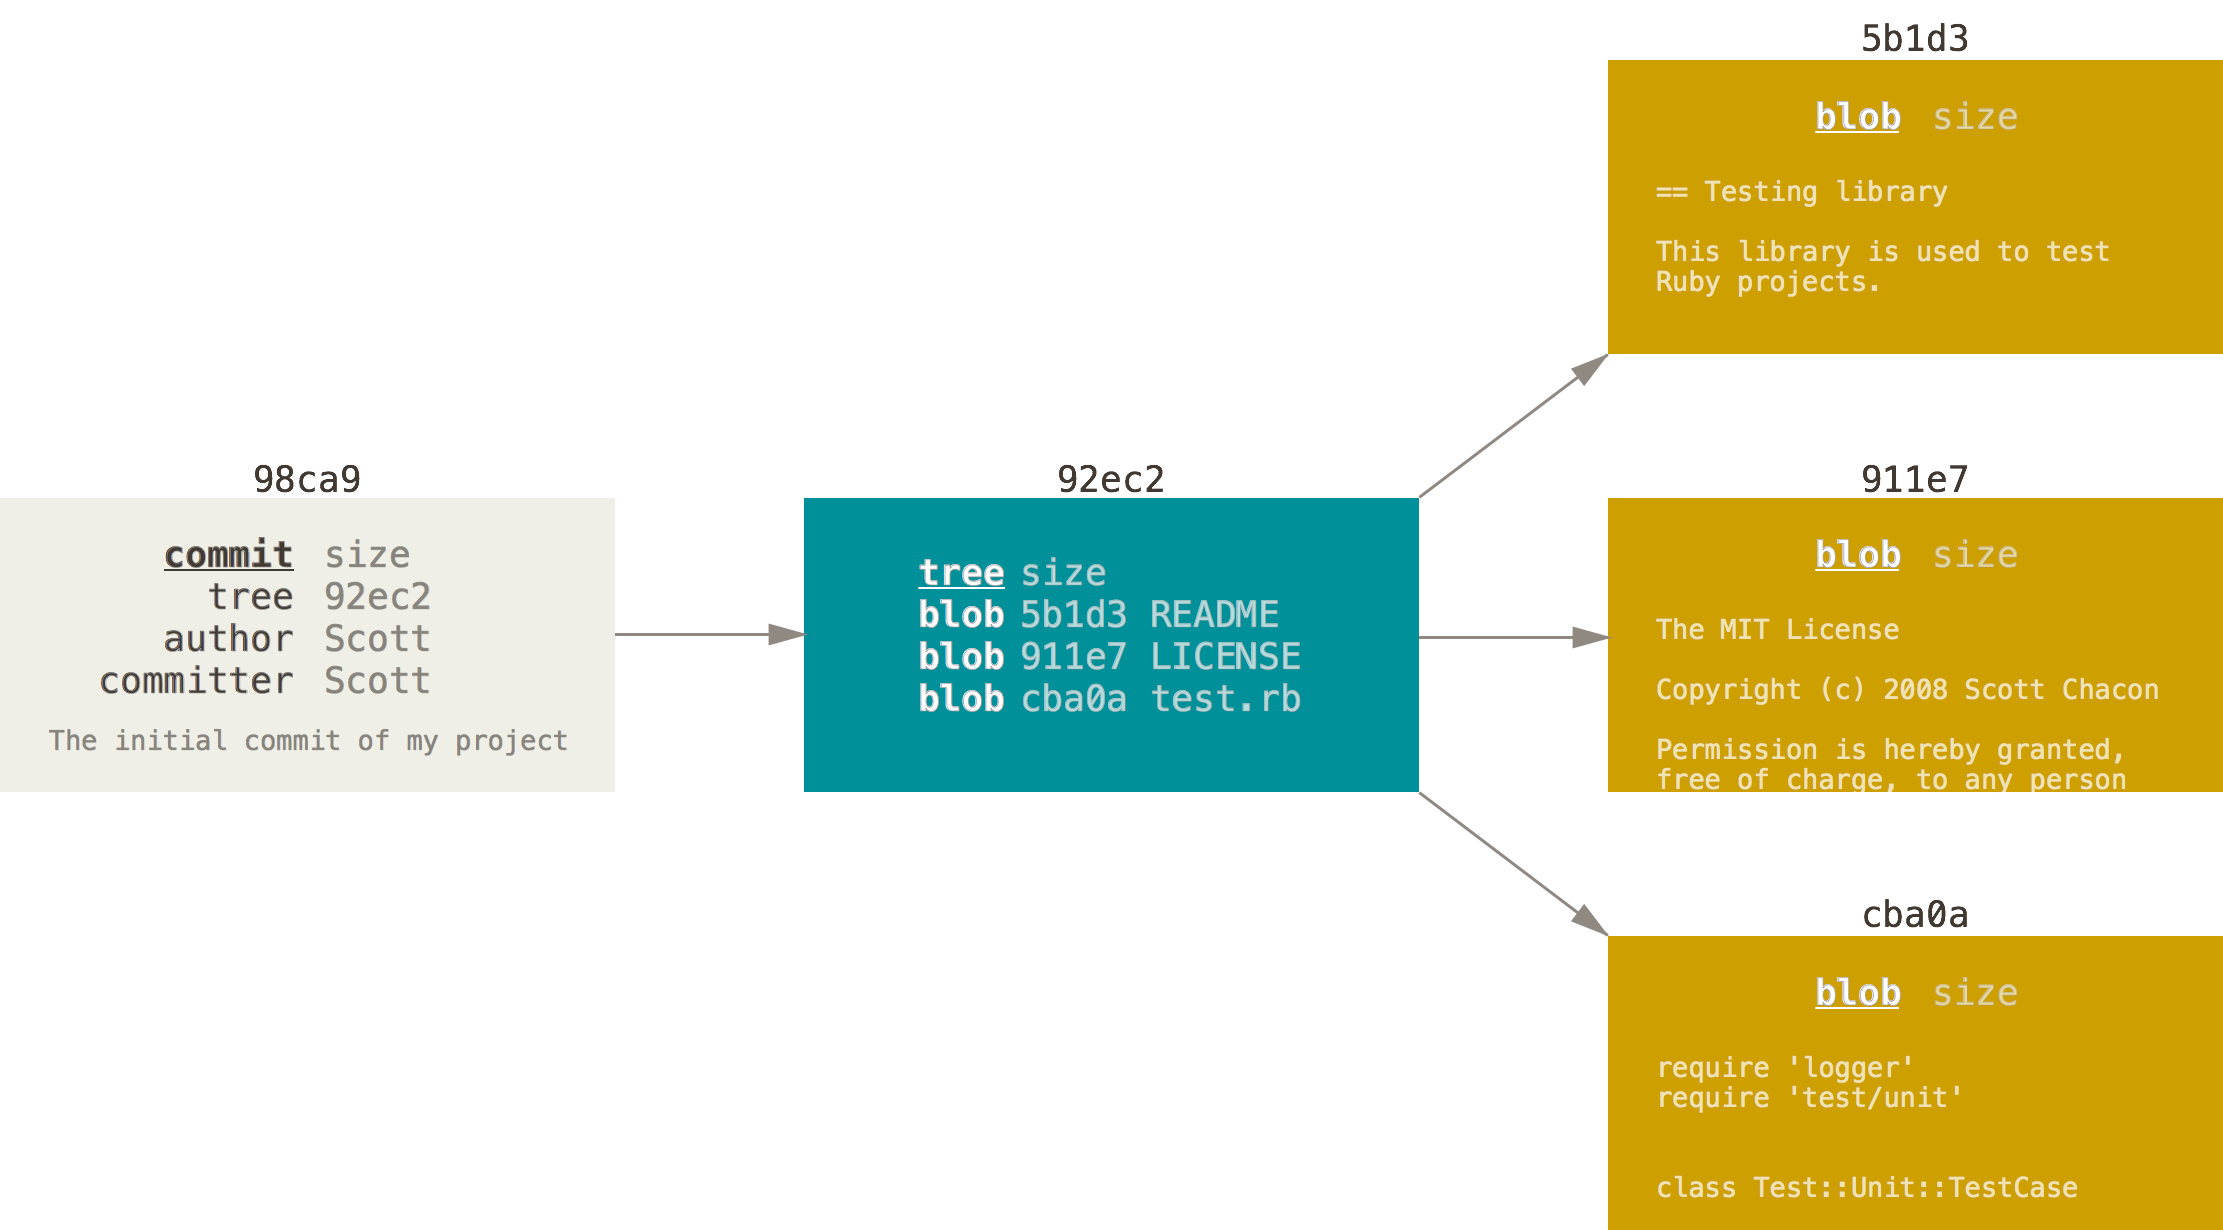
\includegraphics{images/commit-and-tree}
  \caption{Un commit et son arbre}
  \label{fig:git:commit-and-tree}
\end{figure}

Si vous faites des modifications et validez à nouveau, le prochain \emph{commit} stocke un pointeur vers le \emph{commit} le précédant immédiatement.

\begin{figure}[H]
  \centering
  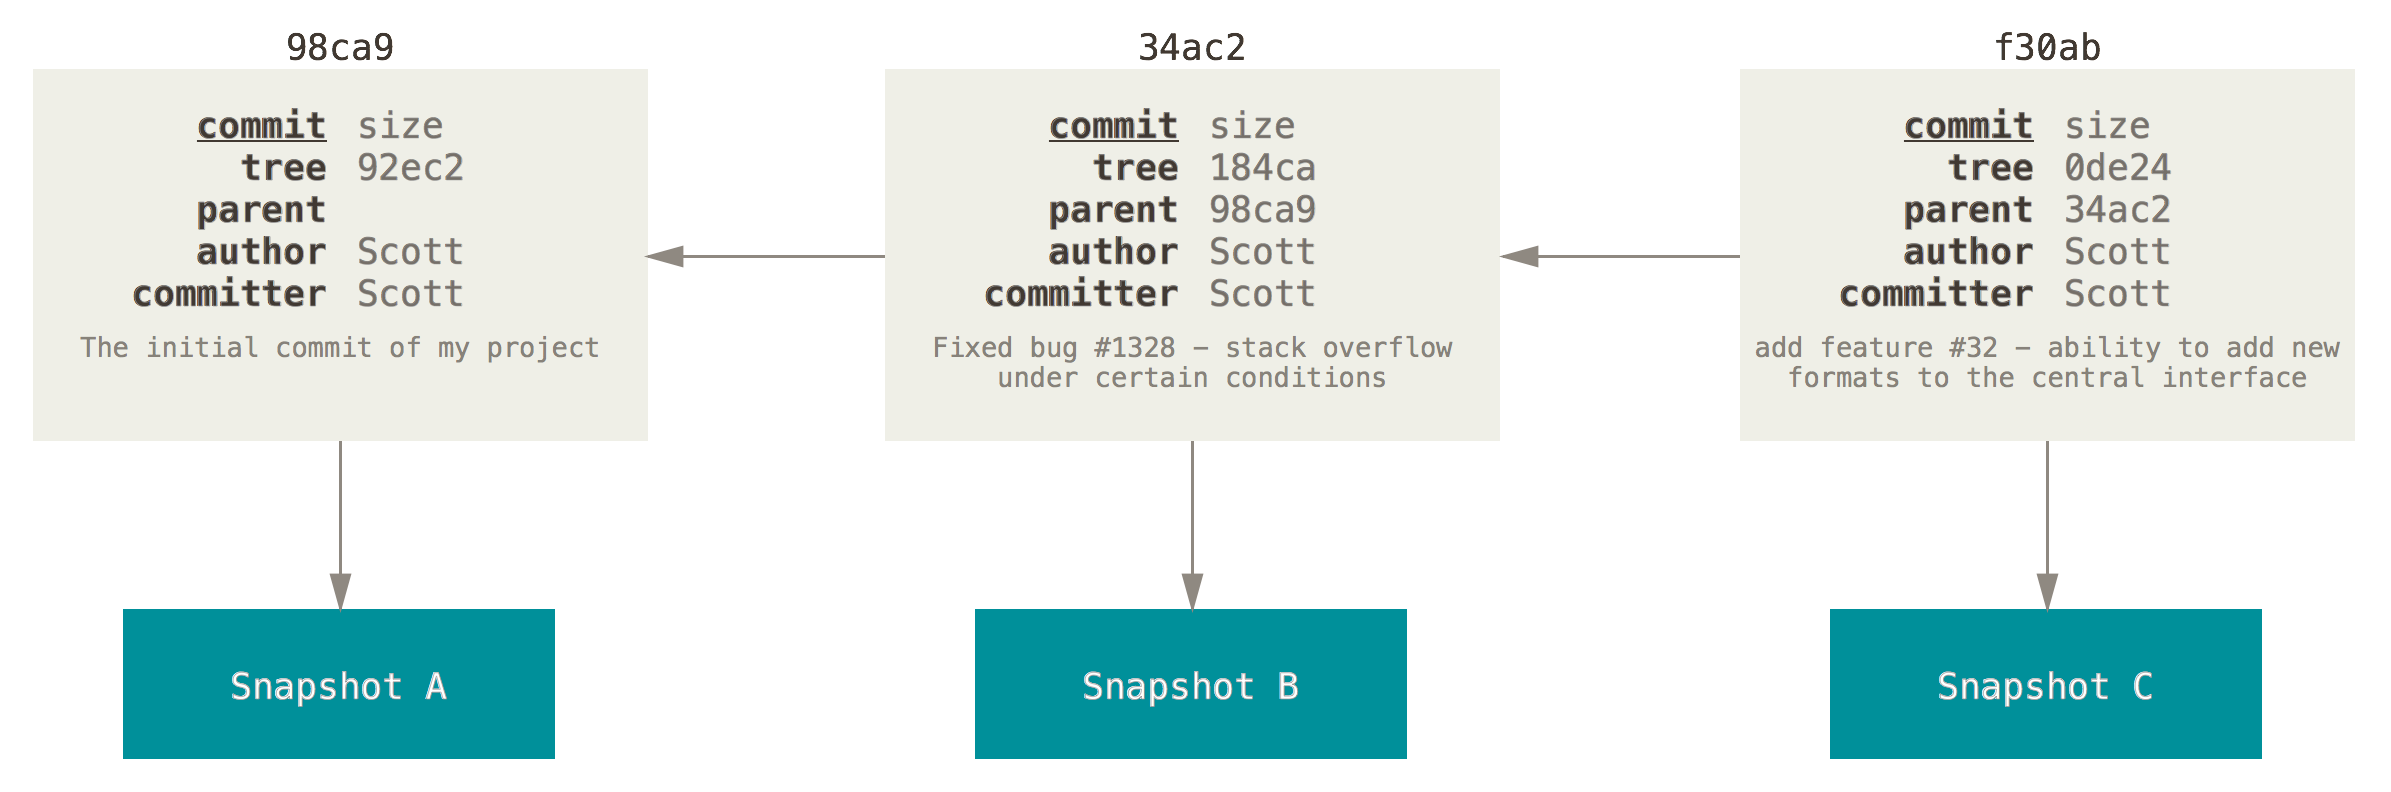
\includegraphics{images/commits-and-parents}
  \caption{Commits et leurs parents}
  \label{fig:git:commits-and-parents}
\end{figure}

Une branche dans Git est simplement un pointeur léger et déplaçable vers un de ces \emph{commits}.
La branche par défaut dans Git s'appelle \code{master}.
Au fur et à mesure des validations, la branche \code{master} pointe vers le dernier des \emph{commits} réalisés.
À chaque validation, le pointeur de la branche \code{master} avance automatiquement.

\notebox{La branche \code{master} n'est pas une branche spéciale.
Elle est identique à toutes les autres branches.
La seule raison pour laquelle chaque dépôt en a une est que la commande \code{git init} la crée par défaut et que la plupart des gens ne s'embêtent pas à la changer.}

\begin{figure}[H]
  \centering
  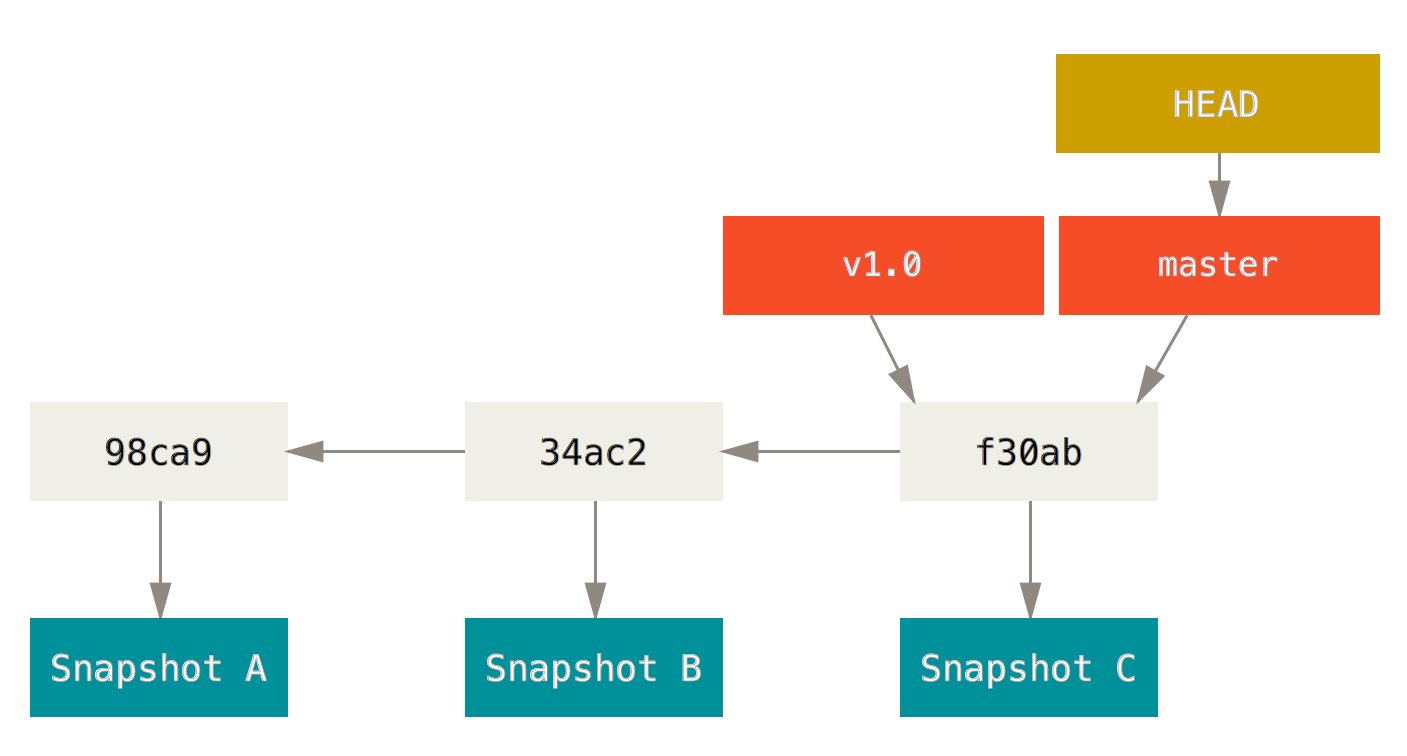
\includegraphics{images/branch-and-history}
  \caption{Une branche et l'historique de ses \emph{commits}}
  \label{fig:git:branch-and-history}
\end{figure}

\subsubsection{Créer une nouvelle branche}
\label{sec:git:create_new_branch}

Que se passe-t-il si vous créez une nouvelle branche?
Eh bien, cela crée un nouveau pointeur pour vous.
Supposons que vous créez une nouvelle branche nommée \code{test}.
Vous utilisez pour cela la commande \code{git branch}:
\begin{Schunk}
\begin{Verbatim}
$ git branch testing
\end{Verbatim}
\end{Schunk}

Cela crée un nouveau pointeur vers le \emph{commit} courant.

\begin{figure}[H]
  \centering
  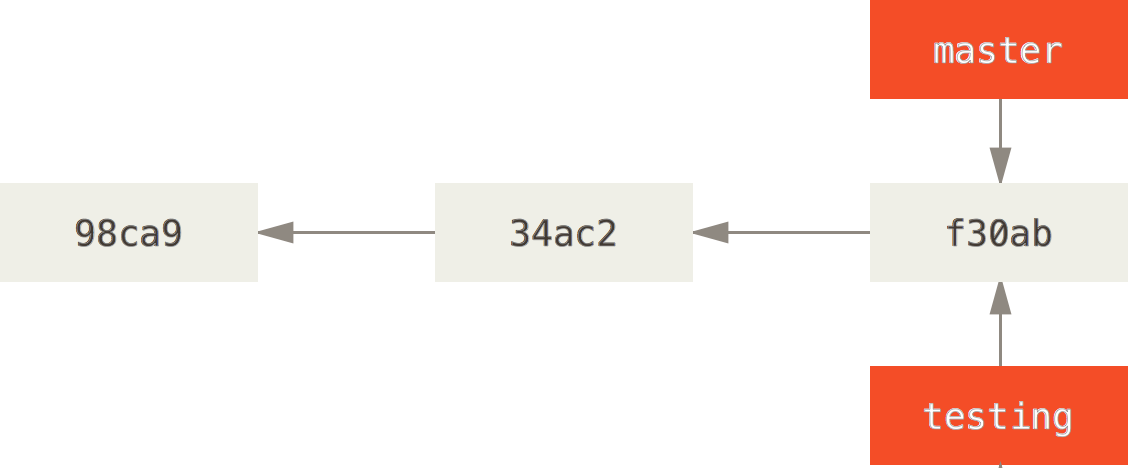
\includegraphics{images/two-branches}
  \caption{Deux branches pointant vers la même série de \emph{commits}}
  \label{fig:git:two-branches}
\end{figure}

Comment Git connaît-il alors la branche sur laquelle vous vous trouvez?
Il conserve à cet effet un pointeur spécial appelé \code{HEAD}.
Vous remarquez que sous cette appellation se cache un concept très différent de celui utilisé dans les autres VCS tels que Subversion ou CVS.
Dans Git, il s'agit simplement d'un pointeur sur la branche locale où vous vous trouvez.
Dans ce cas, vous vous trouvez toujours sur \code{master}.
En effet, la commande \code{git branch} n'a fait que créer une nouvelle branche — elle n'a pas fait basculer la copie de travail vers cette branche.

\begin{figure}[H]
  \centering
  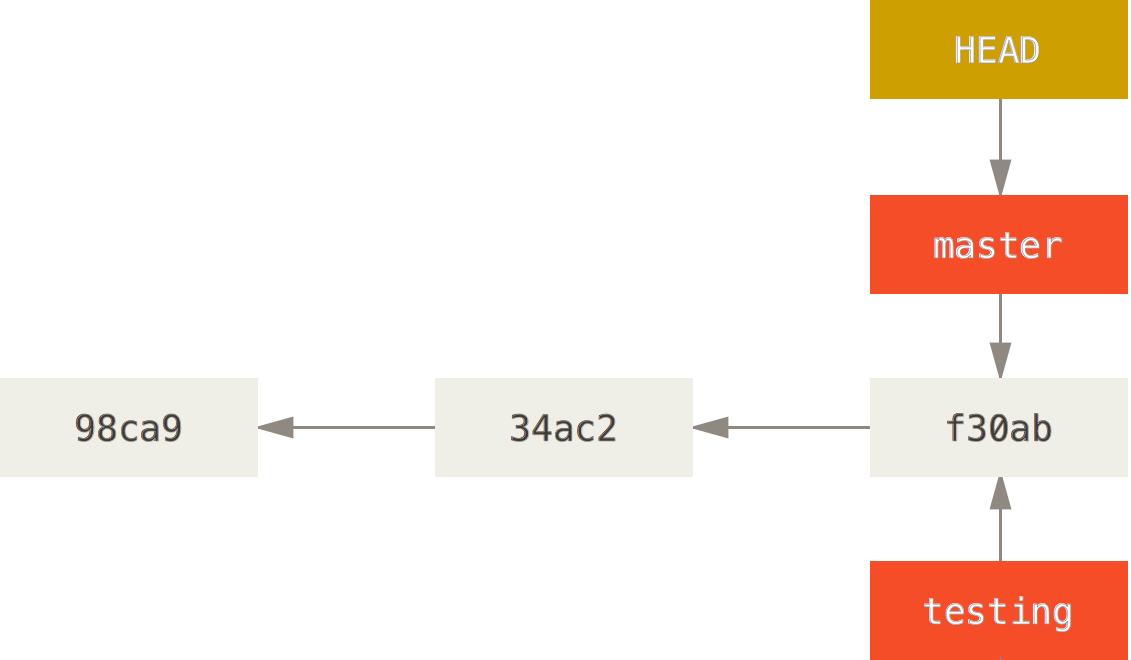
\includegraphics{images/head-to-master}
  \caption{HEAD pointant vers une branche}
  \label{fig:git:head-to-master}
\end{figure}

Vous pouvez vérifier cela facilement grâce à la commande \code{git log} qui vous montre vers quoi les branches pointent. Il s'agit de l'option \code{--decorate}.
\begin{Schunk}
\begin{Verbatim}[commandchars=\\\{\}]
$ git log --oneline --decorate
f30ab (HEAD, master, test) add feature #32 - ability to\meta{...}
34ac2 fixed bug #1328 - stack overflow under certain co\meta{...}
98ca9 initial commit of my project
\end{Verbatim}
\end{Schunk}

Vous pouvez voir les branches \code{master}  et \code{test} qui se situent au niveau du \emph{commit} \code{f30ab}.

\subsubsection{Basculer entre les branches}
\label{sec:git:switching_branches}

Pour basculer sur une branche existante, il suffit de lancer la commande \code{git checkout}.
Basculons sur la nouvelle branche \code{testing}:
\begin{Schunk}
\begin{Verbatim}
$ git checkout testing
\end{Verbatim}
\end{Schunk}

Cela déplace \code{HEAD} pour le faire pointer vers la branche \code{testing}.

\begin{figure}[H]
  \centering
  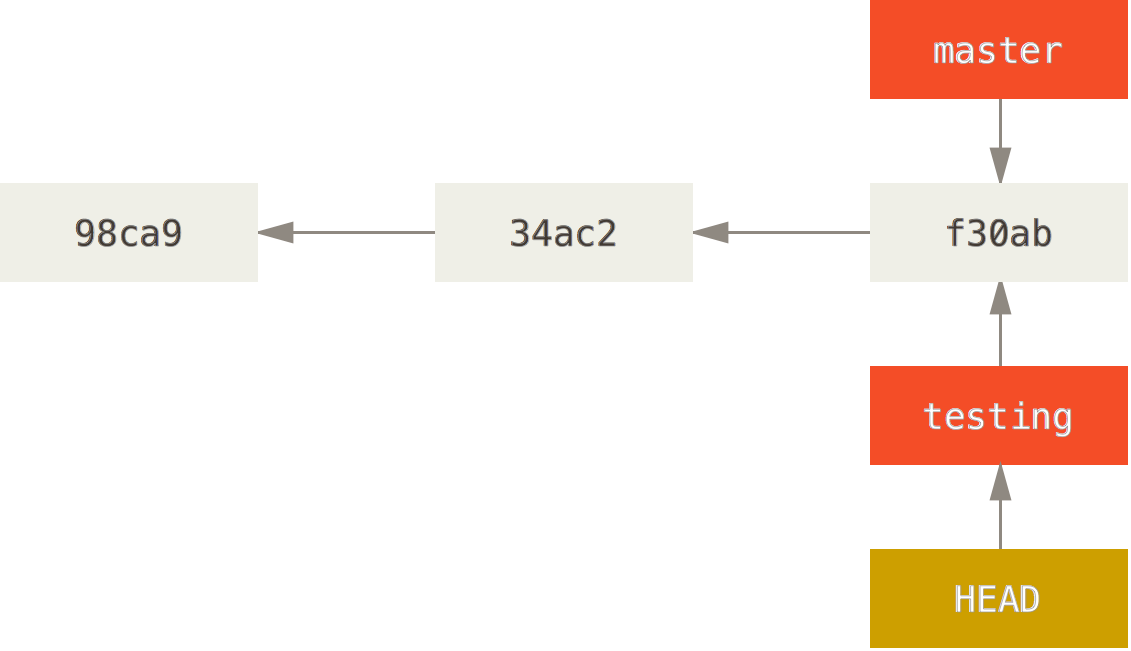
\includegraphics{images/head-to-testing}
  \caption{HEAD pointe vers la branche courante}
  \label{fig:git:head-to-testing}
\end{figure}

Qu'est-ce que cela signifie?
Et bien, faisons une autre validation:
\begin{Schunk}
\begin{Verbatim}
$ vim test.rb
$ git commit -a -m 'made a change'
\end{Verbatim}
\end{Schunk}

\begin{figure}[H]
  \centering
  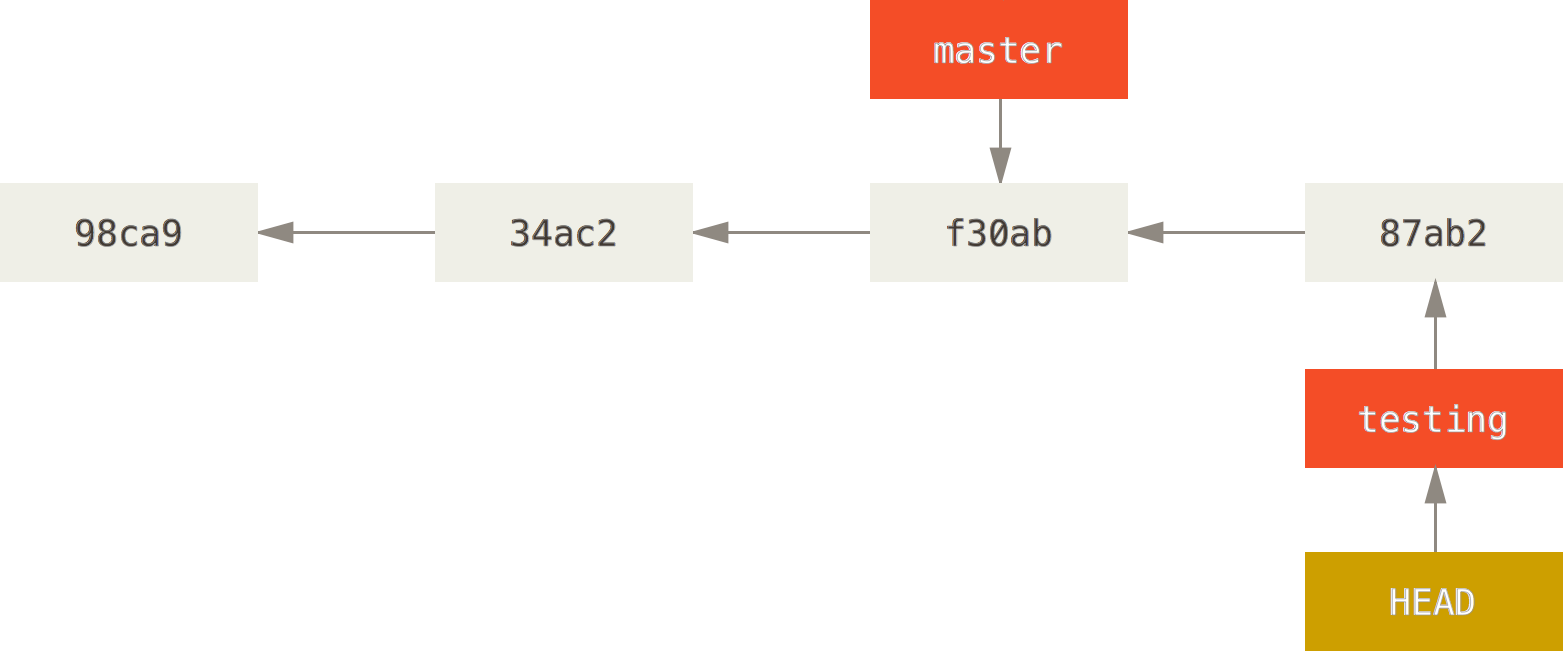
\includegraphics{images/advance-testing}
  \caption{La branche HEAD avance à chaque \emph{commit}}
  \label{fig:git:advance-testing}
\end{figure}

C'est intéressant parce qu'à présent, votre branche \code{test} a avancé tandis que la branche \code{master} pointe toujours sur le \emph{commit} sur lequel vous étiez lorsque vous avez lancé la commande \code{git checkout} pour changer de branche.
Retournons sur la branche \code{master}:
\begin{Schunk}
\begin{Verbatim}
$ git checkout master
\end{Verbatim}
\end{Schunk}

\begin{figure}[H]
  \centering
  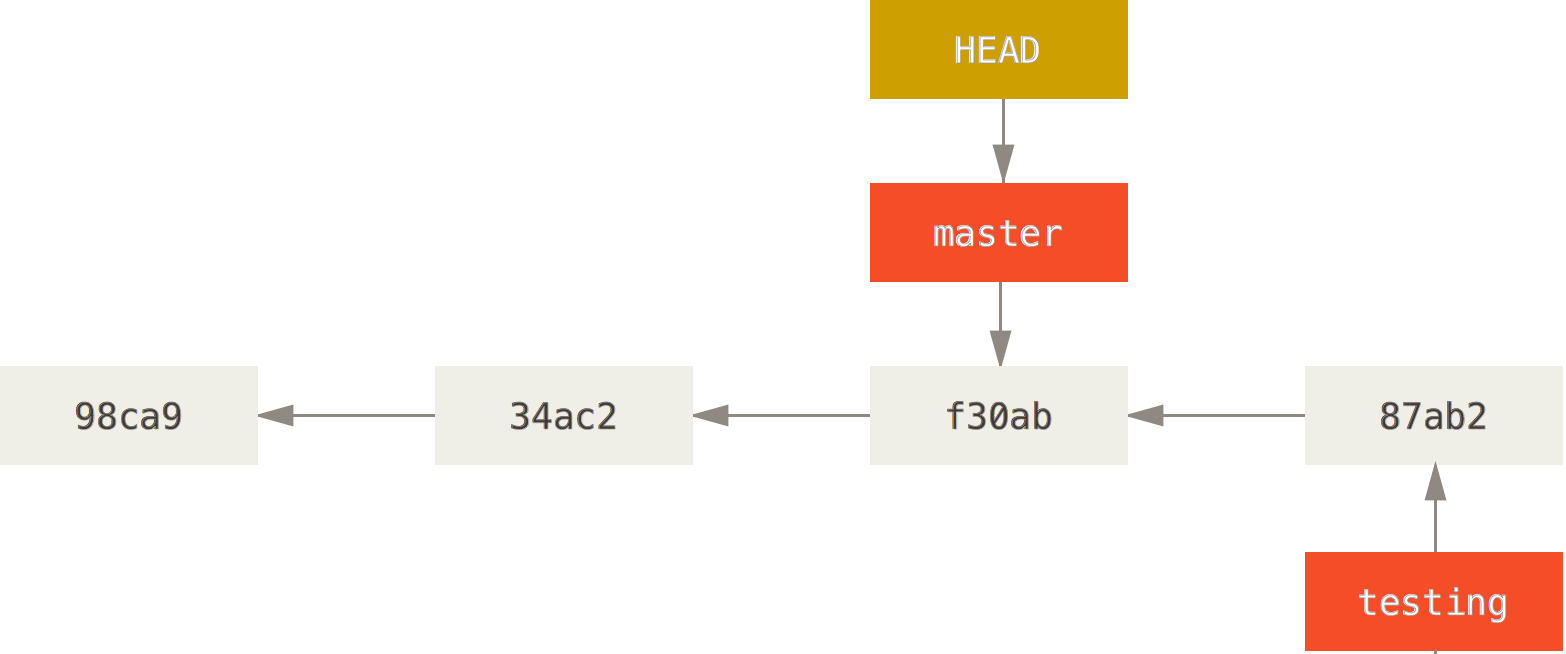
\includegraphics{images/checkout-master}
  \caption{HEAD est déplacé lors d'un \emph{checkout}}
  \label{fig:git:checkout-master}
\end{figure}

Cette commande a réalisé deux actions.
Elle a remis le pointeur \code{HEAD} sur la branche \code{master} et elle a replacé les fichiers de votre répertoire de travail dans l'état du \emph{snapshot} pointé par \code{master}.
Cela signifie aussi que les modifications que vous réalisez à partir de ce point divergeront de l'ancienne version du projet.
Cette commande annule les modifications réalisées dans la branche \code{test} pour vous permettre de repartir dans une autre direction.

\notebox{Il est important de noter que lorsque vous changez de branche avec Git, les fichiers de votre répertoire de travail sont modifiés.
Si vous basculez vers une branche plus ancienne, votre répertoire de travail sera remis dans l'état dans lequel il était lors du dernier \emph{commit} sur cette branche.
Si Git n'est pas en mesure d'effectuer cette action proprement, il ne vous laissera pas changer de branche.}

Réalisons quelques autres modifications et validons à nouveau:
\begin{Schunk}
\begin{Verbatim}
$ vim test.rb
$ git commit -a -m 'made other changes'
\end{Verbatim}
\end{Schunk}

Maintenant, l'historique du projet a divergé (voir la \autoref{fig:git:divergent_history}).
Vous avez créé une branche et basculé dessus, y avez réalisé des modifications, puis vous avez rebasculé sur la branche principale et réalisé d'autres modifications.
Ces deux modifications sont isolées dans des branches séparées: vous pouvez basculer d'une branche à l'autre et les fusionner quand vous êtes prêt.
Et vous avez fait tout ceci avec de simples commandes: \code{branch}, \code{checkout} et \code{commit}.

\begin{figure}[H]
  \centering
  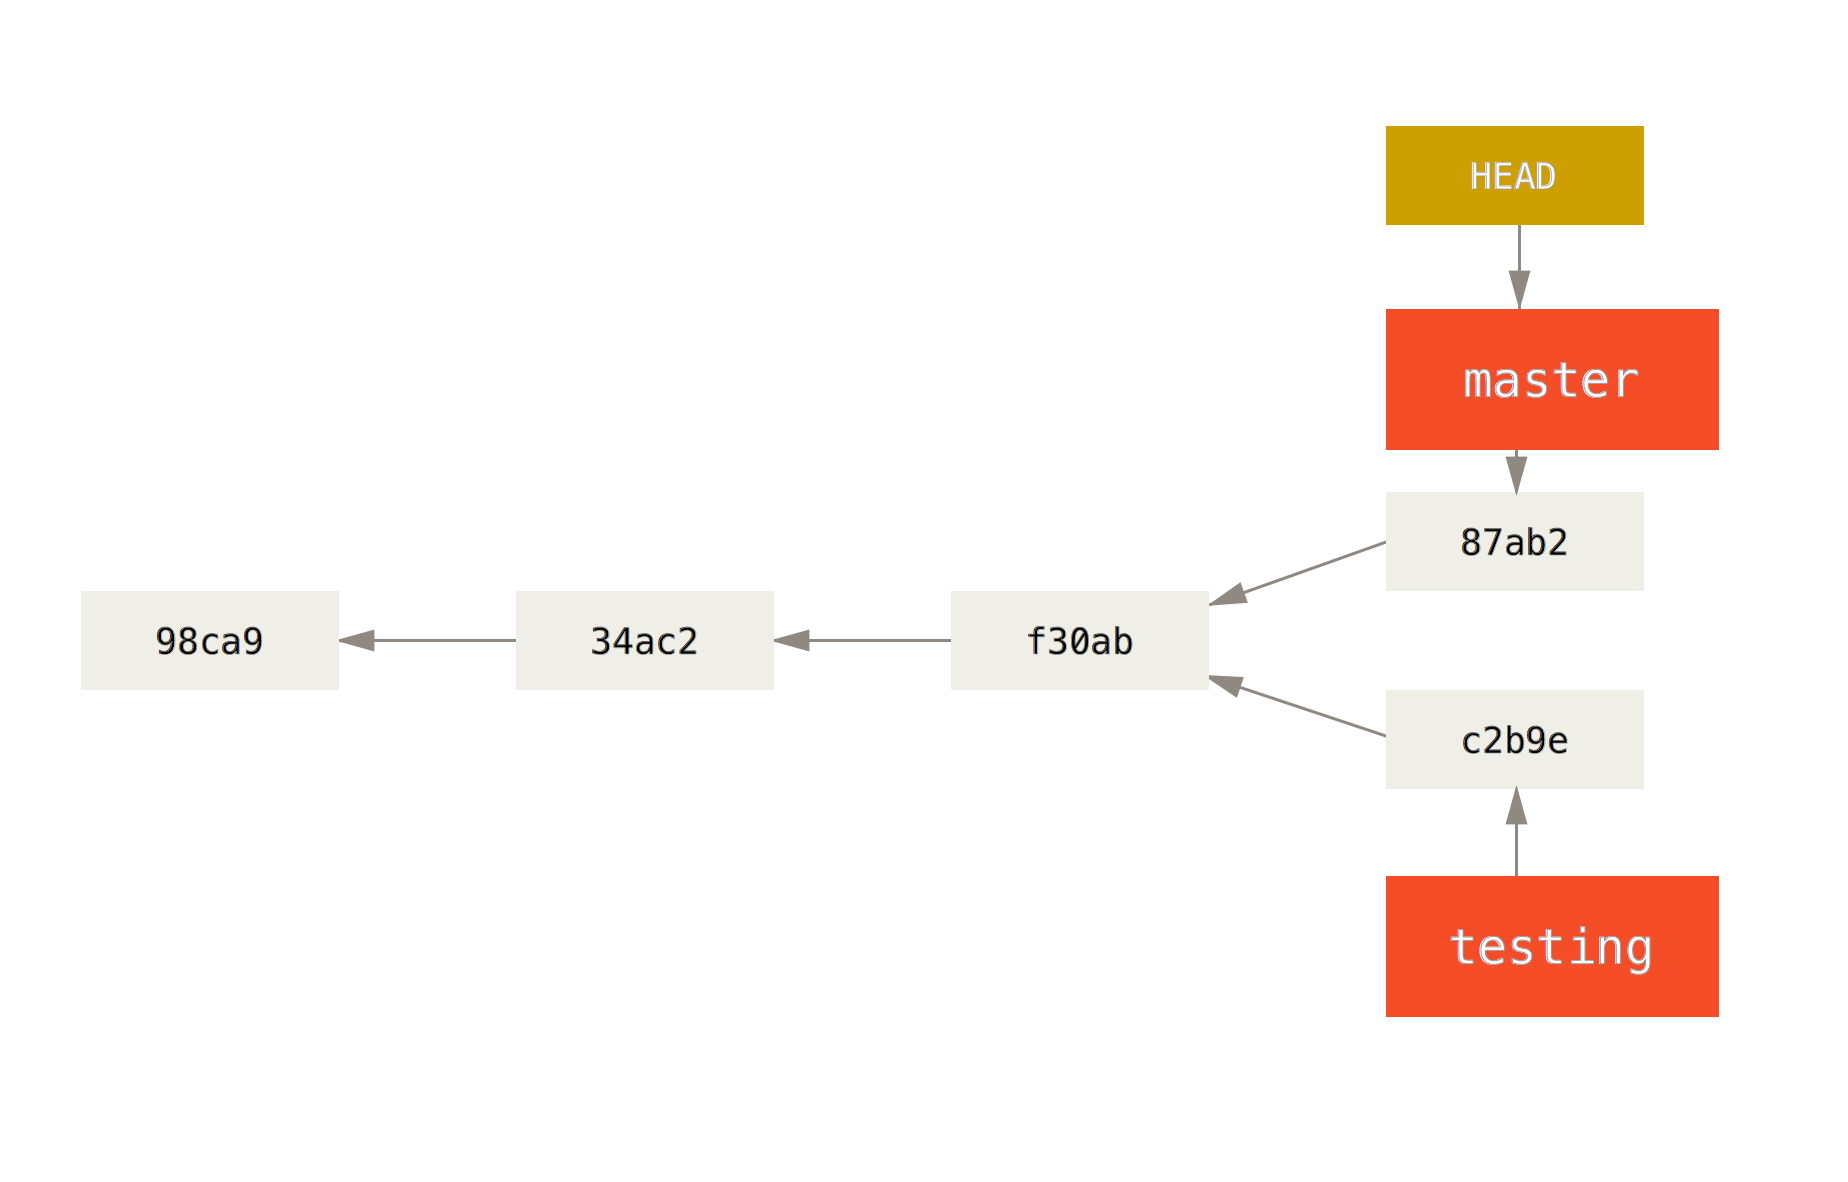
\includegraphics{images/advance-master}
  \caption{Divergence d'historique}
  \label{fig:git:divergent_history}
\end{figure}

Vous pouvez également voir ceci grâce à la commande \code{git log}.
La commande \code{git log --oneline --decorate --graph --all} va afficher l'historique de vos \emph{commits}, affichant les endroits où sont positionnés vos pointeurs de branche ainsi que la manière dont votre historique a divergé.
\begin{Schunk}
\begin{Verbatim}[commandchars=\\\{\}]
$ git log --oneline --decorate --graph --all
* c2b9e (HEAD, master) made other changes
| * 87ab2 (test) made a change
|/
* f30ab add feature #32 - ability to add new formats to the
* 34ac2 fixed bug #1328 - stack overflow under certain \meta{...}
* 98ca9 initial commit of my project
\end{Verbatim}
\end{Schunk}

Parce qu'une branche Git n'est en fait qu'un simple fichier contenant les 40 caractères de l'empreinte SHA-1 du \emph{commit} sur lequel elle pointe, les branches ne coûtent quasiment rien à créer et à détruire.
Créer une branche est aussi simple et rapide qu'écrire 41 caractères dans un fichier (40 caractères plus un retour chariot).

C'est une différence de taille avec la manière dont la plupart des VCS gèrent les branches, qui implique de copier tous les fichiers du projet dans un second répertoire.
Cela peut durer plusieurs secondes ou même quelques minutes selon la taille du projet, alors que pour Git, le processus est toujours instantané.
De plus, comme nous enregistrons les parents quand nous validons les modifications, la détermination de l'ancêtre commun approprié pour la fusion est réalisée automatiquement pour nous et est généralement une opération très facile.
Ces fonctionnalités encouragent naturellement les développeurs à créer et utiliser souvent des branches.

Voyons pourquoi vous devriez en faire autant.

\subsection{Branches et fusions: les bases}

Prenons un exemple simple faisant intervenir des branches et des fusions (\emph{merges}) que vous pourriez trouver dans le monde réel.
Vous effectuez les tâches suivantes:

\begin{itemize}
\item vous travaillez sur un site web;
\item vous créez une branche pour un nouvel article en cours;
\item vous commencez à travailler sur cette branche.
\end{itemize}

À cette étape, vous recevez un appel pour vous dire qu'un problème critique a été découvert et qu'il faut le régler au plus tôt.
Vous faites donc ce qui suit:

\begin{itemize}
\item vous basculez sur la branche de production;
\item vous créez une branche pour y ajouter le correctif;
\item après l'avoir testé, vous fusionnez la branche du correctif et poussez le résultat en production;
\item vous rebasculez sur la branche initiale et continuez votre travail.
\end{itemize}

\subsubsection{Branches}
\label{sec:git:basic_branching}

Commençons par supposer que vous travaillez sur votre projet et avez déjà quelques \emph{commits}.

\begin{figure}[H]
  \centering
  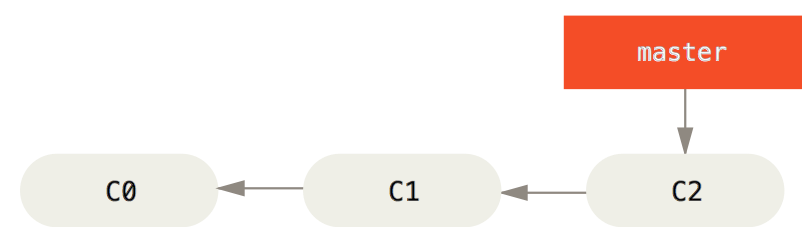
\includegraphics{images/basic-branching-1}
  \caption{Historique de \emph{commits} simple}
  \label{fig:git:basic-branching-1}
\end{figure}

Vous avez décidé de travailler sur le problème numéroté \#53 dans l'outil de gestion des tâches que votre entreprise utilise, quel qu'il soit.
Pour créer une branche et y basculer tout de suite, vous pouvez lancer la commande \code{git checkout} avec l'option \code{-b}:
\begin{Schunk}
\begin{Verbatim}
$ git checkout -b prob53
Switched to a new branch "prob53"
\end{Verbatim}
\end{Schunk}

Cette commande est un raccourci pour:
\begin{Schunk}
\begin{Verbatim}
$ git branch prob53
$ git checkout prob53
\end{Verbatim}
\end{Schunk}

\begin{figure}[H]
  \centering
  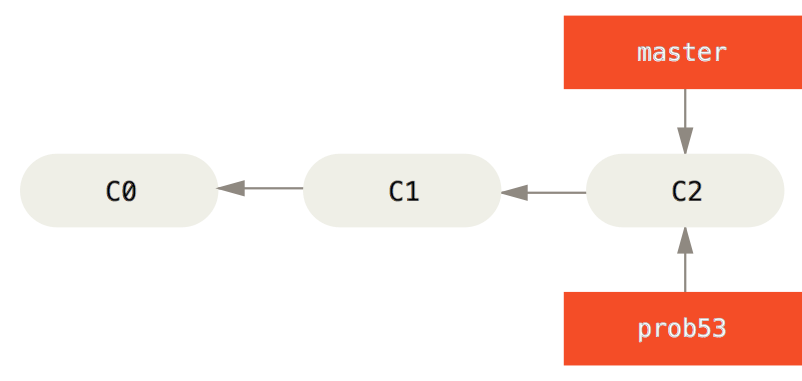
\includegraphics{images/basic-branching-2}
  \caption{Création d'un nouveau pointeur de branche}
  \label{fig:git:basic-branching-2}
\end{figure}

Vous travaillez sur votre site web et validez vos modifications.
Ce faisant, la branche \code{prob53} avance parce que vous l'avez extraite (c'est-à-dire que votre pointeur \code{HEAD} pointe dessus):
\begin{Schunk}
\begin{Verbatim}
$ vim index.html
$ git commit -a -m "ajout d'un pied de page [problème 53]"
\end{Verbatim}
\end{Schunk}

\begin{figure}[H]
  \centering
  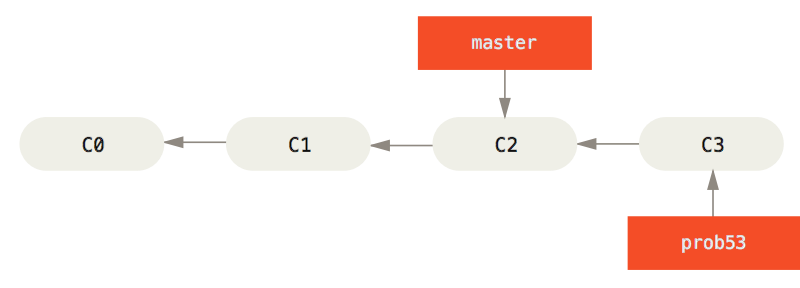
\includegraphics{images/basic-branching-3}
  \caption{La branche \code{prob53} a avancé avec votre travail}
  \label{fig:git:basic-branching-3}
\end{figure}

À ce moment-là, vous recevez un appel qui vous apprend qu'il y a un problème sur le site web qu'il faut résoudre immédiatement.
Avec Git, vous n'avez pas à déployer en même temps votre correctif et les modifications déjà validées pour \code{prob53} et vous n'avez pas non plus à vous fatiguer à annuler ces modifications avant de pouvoir appliquer votre correctif sur ce qu'il y a en production.
Tout ce que vous avez à faire, c'est simplement de rebasculer sur la branche \code{master}.

Cependant, avant de le faire, notez que si votre copie de travail ou votre zone d'index contiennent des modifications non validées qui sont en conflit avec la branche que vous extrayez, Git ne vous laissera pas effectuer le changement de branche.
Le mieux est d'avoir votre copie de travail propre au moment de changer de branche.
Il y a des moyens de contourner ceci (précisément par le remisage et l'amendement de \emph{commit}) dont nous parlerons plus loin, au chapitre \emph{Remisage et nettoyage}.
Pour l'instant, nous supposons que vous avez validé tous vos changements et que vous pouvez donc rebasculer vers votre branche \code{master}:
\begin{Schunk}
\begin{Verbatim}
$ git checkout master
Switched to branch 'master'
\end{Verbatim}
\end{Schunk}

À cet instant, votre répertoire de copie de travail est exactement dans l'état dans lequel vous l'aviez laissé avant de commencer à travailler sur le problème \#53 et vous pouvez vous consacrer à votre correctif.
C'est un point important à garder en mémoire: quand vous changez de branche, Git réinitialise votre répertoire de travail pour qu'il soit le même que la dernière fois que vous avez effectué un \emph{commit} sur cette branche.
Il ajoute, retire et modifie automatiquement les fichiers de manière à s'assurer que votre copie de travail soit identique à ce qu'elle était lors de votre dernier \emph{commit} sur cette branche.

Vous avez ensuite un correctif à faire.
Pour ce faire, créons une branche \code{correctif} sur laquelle travailler jusqu'à résolution du problème:
\begin{Schunk}
\begin{Verbatim}[commandchars=\\\{\}]
$ git checkout -b correctif
Switched to a new branch 'correctif'
$ vim index.html
$ git commit -a
    -m "correction de l'adresse email incorrecte"
[correctif 1fb7853] "correction de l'adresse email inco\meta{...}
 1 file changed, 2 insertions(+)
\end{Verbatim}
\end{Schunk}

\begin{figure}[H]
  \centering
  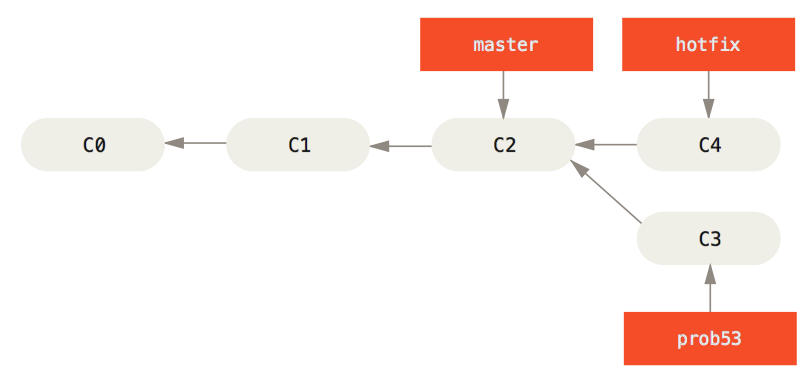
\includegraphics{images/basic-branching-4}
  \caption{Branche de correctif basée sur \code{master}}
  \label{fig:git:basic-branching-4}
\end{figure}

Vous pouvez lancer vos tests, vous assurer que la correction est efficace et la fusionner dans la branche \code{master} pour la déployer en production.
Vous réalisez ceci au moyen de la commande \code{git merge}:
\begin{Schunk}
\begin{Verbatim}
$ git checkout master
$ git merge correctif
Updating f42c576..3a0874c
Fast-forward
 index.html | 2 ++
 1 file changed, 2 insertions(+)
\end{Verbatim}
\end{Schunk}

Vous noterez la mention \code{fast-forward} lors de cette fusion (\emph{merge}).
Comme le \emph{commit} \code{C4} pointé par la branche \code{hotfix} que vous avez fusionnée était directement devant le \emph{commit} \code{C2} sur lequel vous vous trouvez, Git a simplement déplacé le pointeur (vers l'avant).
Autrement dit, lorsque l'on cherche à fusionner un \emph{commit} qui peut être atteint en parcourant l'historique depuis le \emph{commit} d'origine, Git se contente d'avancer le pointeur car il n'y a pas de travaux divergents à fusionner. Ceci s'appelle un \code{fast-forward} (avance rapide).

Votre modification est maintenant dans l'instantané (\emph{snapshot}) du \emph{commit} pointé par la branche \code{master} et vous pouvez déployer votre correctif.

\begin{figure}[H]
  \centering
  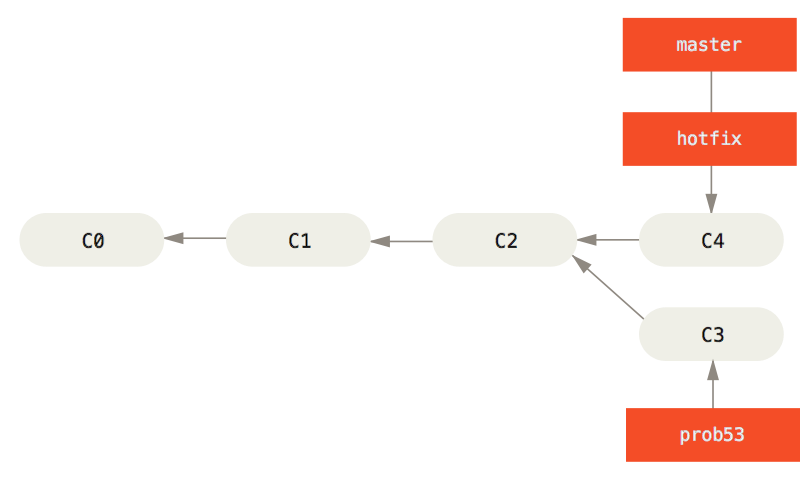
\includegraphics{images/basic-branching-5}
  \caption{Avancement du pointeur de \code{master} sur \code{correctif}}
  \label{fig:git:basic-branching-5}
\end{figure}

Après le déploiement de votre correctif super-important, vous voilà prêt à retourner travailler sur le sujet qui vous occupait avant l'interruption.
Cependant, vous allez avant cela effacer la branche \code{correctif} dont vous n'avez plus besoin puisque la branche \code{master} pointe au même endroit.
Vous pouvez l'effacer avec l'option \code{-d} de la commande \code{git branch}:

\begin{Schunk}
\begin{Verbatim}
$ git branch -d correctif
Deleted branch correctif (3a0874c).
\end{Verbatim}
\end{Schunk}

Maintenant, vous pouvez retourner travailler sur la branche qui contient vos travaux en cours pour le problème \#53:
\begin{Schunk}
\begin{Verbatim}
$ git checkout prob53
Switched to branch "prob53"
$ vim index.html
$ git commit -a -m 'Nouveau pied de page terminé [issue 53]'
[prob53 ad82d7a] Nouveau pied de page terminé [issue 53]
1 file changed, 1 insertion(+)
\end{Verbatim}
\end{Schunk}

\begin{figure}[H]
  \centering
  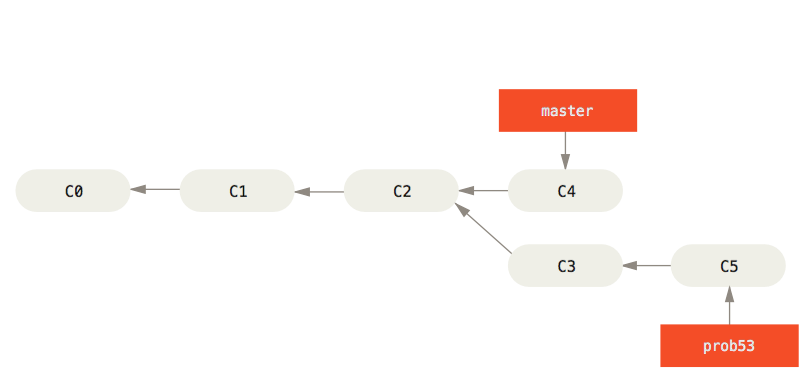
\includegraphics{images/basic-branching-6}
  \caption{Le travail continue sur \code{prob53}}
  \label{fig:git:basic-branching-6}
\end{figure}

Il est utile de noter que le travail réalisé dans la branche \code{correctif} n'est pas contenu dans les fichiers de la branche \code{prob53}.
Si vous avez besoin de les y rapatrier, vous pouvez fusionner la branche \code{master} dans la branche \code{prob53} en lançant la commande \code{git merge master}, ou vous pouvez retarder l'intégration de ces modifications jusqu'à ce que vous décidiez plus tard de rapatrier la branche \code{prob53} dans \code{master}.


\subsubsection{Fusions (\emph{Merges})}
\label{sec:git:basic_merging}

Supposons que vous ayez décidé que le travail sur le problème \#53 était terminé et prêt à être fusionné dans la branche \code{master}.
Pour ce faire, vous allez fusionner votre branche \code{prob53} de la même manière que vous l'avez fait plus tôt pour la branche \code{correctif}.
Tout ce que vous avez à faire est d'extraire la branche dans laquelle vous souhaitez fusionner et lancer la commande \code{git merge}:
\begin{Schunk}
\begin{Verbatim}
$ git checkout master
Switched to branch 'master'
$ git merge prob53
Merge made by the 'recursive' strategy.
README |    1 +
1 file changed, 1 insertion(+)
\end{Verbatim}
\end{Schunk}

Le comportement semble légèrement différent de celui observé pour la fusion précédente de la branche \code{correctif}.
Dans ce cas, à un certain moment, l'historique de développement a divergé.
Comme le \emph{commit} sur la branche sur laquelle vous vous trouvez n'est plus un ancêtre direct de la branche que vous cherchez à fusionner, Git doit effectuer quelques actions.
Dans ce cas, Git réalise une simple fusion à trois sources (\emph{three-way merge}), en utilisant les deux instantanés pointés par les sommets des branches ainsi que leur plus proche ancêtre commun.

\begin{figure}[H]
  \centering
  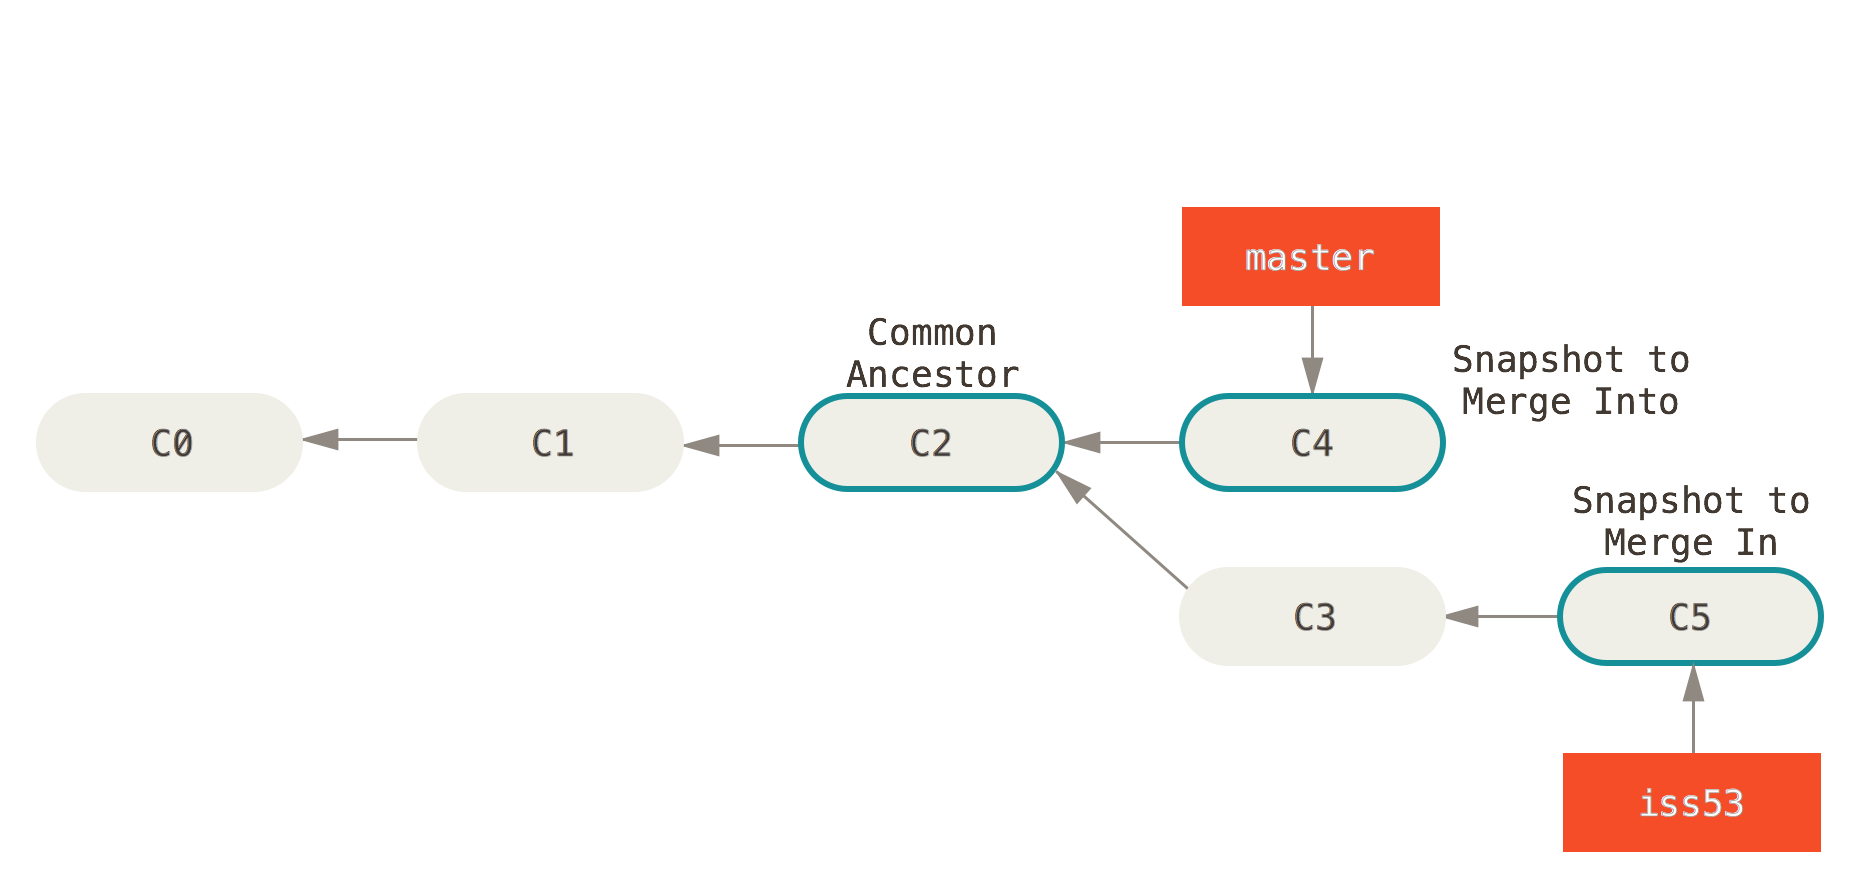
\includegraphics{images/basic-merging-1}
  \caption{Trois instantanés utilisés dans une fusion classique}
  \label{fig:git:basic-merging-1}
\end{figure}

Au lieu d'avancer simplement le pointeur de branche, Git crée un nouvel instantané qui résulte de la fusion à trois sources et crée automatiquement un nouveau \emph{commit} qui pointe dessus.
On appelle ceci un \emph{commit} de fusion (\emph{merge commit}) qui est spécial en cela qu'il a plus d'un parent.

\begin{figure}[H]
  \centering
  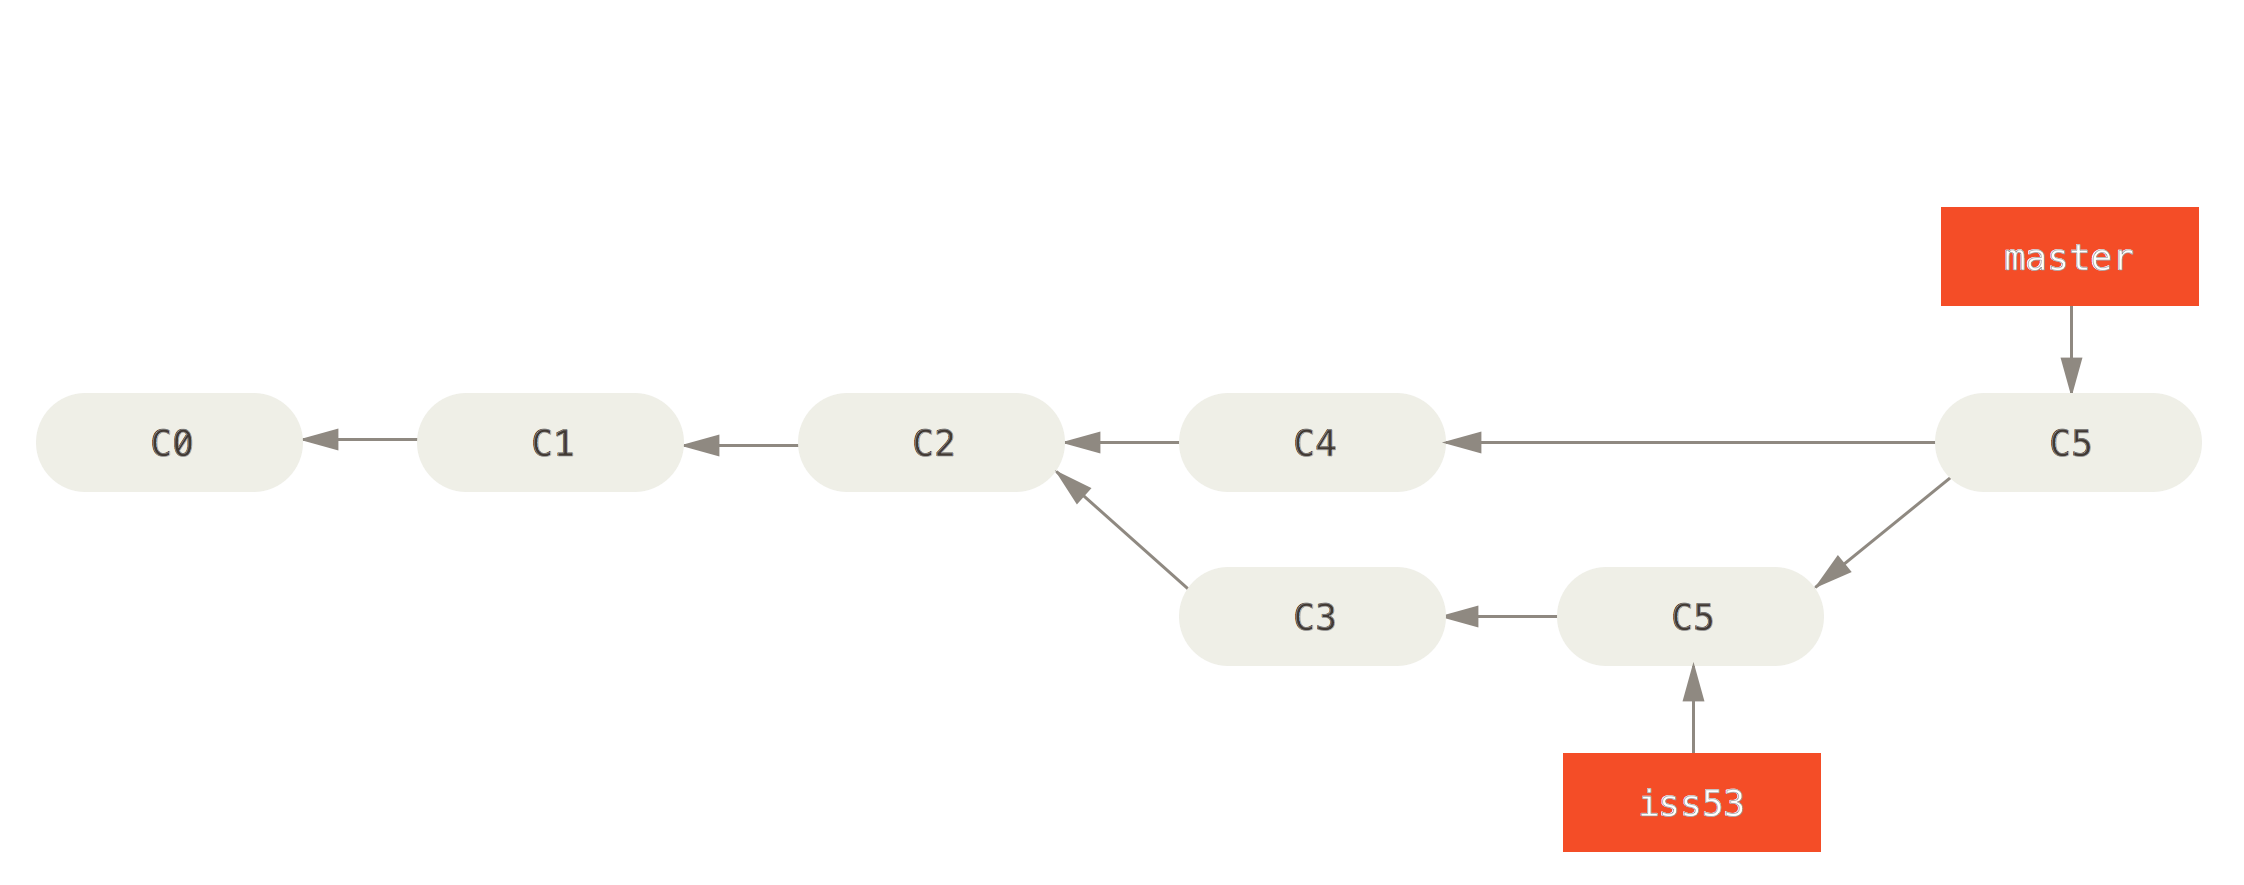
\includegraphics{images/basic-merging-2}
  \caption{Un \emph{commit} de fusion}
  \label{fig:git:basic-merging-2}
\end{figure}

Il est à noter que Git détermine par lui-même le meilleur ancêtre commun à utiliser comme base de la fusion. Ce comportement est très différent de celui de CVS ou Subversion (avant la version 1.5), où le développeur en charge de la fusion doit trouver par lui-même la meilleure base.
Cela rend la fusion beaucoup plus facile dans Git que dans les autres systèmes.

À présent que votre travail a été fusionné, vous n'avez plus besoin de la branche \code{prob53}.
Vous pouvez fermer le ticket dans votre outil de suivi des tâches et supprimer la branche:
\begin{Schunk}
\begin{Verbatim}
$ git branch -d prob53
\end{Verbatim}
\end{Schunk}

\subsubsection{Conflits de fusions (\emph{Merge conflicts})}
\label{sec:git:basic_merge_conflicts}

Quelques fois, le processus ci-dessus ne se déroule pas aussi bien.
Si vous avez modifié différemment la même partie du même fichier dans les deux branches que vous souhaitez fusionner, Git ne sera pas capable de réaliser proprement la fusion.
Si votre résolution du problème \#53 a modifié la même section de fichier que le \code{correctif}, vous obtiendrez un conflit qui ressemblera à ceci:
\begin{Schunk}
\begin{Verbatim}
$ git merge prob53
Auto-merging index.html
CONFLICT (content): Merge conflict in index.html
Automatic merge failed; fix conflicts and then commit
the result.
\end{Verbatim}
\end{Schunk}

Git n'a pas automatiquement créé le \emph{commit} de fusion.
Il a arrêté le processus le temps que vous résolviez le conflit.
Si vous voulez vérifier, à tout moment après l'apparition du conflit, quels fichiers n'ont pas été fusionnés, vous pouvez lancer la commande \code{git status}:
\begin{Schunk}
\begin{Verbatim}
$ git status
On branch master
You have unmerged paths.
  (fix conflicts and run "git commit")

Unmerged paths:
  (use "git add <file>..." to mark resolution)

    both modified:      index.html

no changes added to commit (use "git add" and/or
"git commit -a")
\end{Verbatim}
\end{Schunk}

Tout ce qui comporte des conflits et n'a pas été résolu est listé comme \code{unmerged}.
Git ajoute des marques de résolution de conflit standards dans les fichiers qui comportent des conflits, pour que vous puissiez les ouvrir et résoudre les conflits manuellement.
Votre fichier contient des sections qui ressemblent à ceci:
\begin{Schunk}
\begin{Verbatim}
<<<<<<< HEAD:index.html
<div id="footer">contact: email.support@github.com</div>
=======
<div id="footer">
 please contact us at support@github.com
</div>
>>>>>>> prob53:index.html
\end{Verbatim}
\end{Schunk}

Cela signifie que la version dans \code{HEAD} (votre branche \code{master}, parce que c'est celle que vous aviez extraite quand vous avez lancé votre commande de fusion) est la partie supérieure de ce bloc (tout ce qui se trouve au-dessus de la ligne \code{=======}), tandis que la version de votre branche \code{prob53} se trouve en dessous.
Pour résoudre le conflit, vous devez choisir une partie ou l'autre ou bien fusionner leurs contenus vous-même.
Par exemple, vous pourriez choisir de résoudre ce conflit en remplaçant tout le bloc par ceci:
\begin{Schunk}
\begin{Verbatim}
<div id="footer">
please contact us at email.support@github.com
</div>
\end{Verbatim}
\end{Schunk}

Cette résolution comporte des éléments de chaque section et les lignes \code{<<<<<<<}, \code{=======} et \code{>>>>>>>} ont été complètement effacées.
Après avoir résolu chacune de ces sections dans chaque fichier comportant un conflit, lancez \code{git add} sur chaque fichier pour le marquer comme résolu.
Placer le fichier dans l'index marque le conflit comme résolu pour Git.

Si vous souhaitez utiliser un outil graphique pour résoudre ces conflits, vous pouvez lancer \code{git mergetool} qui démarre l'outil graphique de fusion approprié et vous permet de naviguer dans les conflits:
\begin{Schunk}
\begin{Verbatim}
$ git mergetool

This message is displayed because 'merge.tool' is not
configured.
See 'git mergetool --tool-help' or 'git help config' for
more details.
'git mergetool' will now attempt to use one of the
following tools:
opendiff kdiff3 tkdiff xxdiff meld tortoisemerge gvimdiff
diffuse diffmerge ecmerge p4merge araxis bc3 codecompare
vimdiff emerge
Merging:
index.html

Normal merge conflict for 'index.html':
  {local}: modified file
  {remote}: modified file
Hit return to start merge resolution tool (opendiff):
\end{Verbatim}
\end{Schunk}

Si vous souhaitez utiliser un outil de fusion autre que celui par défaut (Git a choisi \code{opendiff} dans ce cas car la commande a été lancée depuis un Mac), vous pouvez voir tous les outils supportés après l'indication «\emph{of the following tools:}».
Entrez simplement le nom de l'outil que vous préféreriez utiliser.

\notebox{Si vous avez besoin d'outils plus avancés pour résoudre des conflits complexes, vous trouverez davantage d'informations au chapitre \emph{Fusion avancée}.}

Après avoir quitté l'outil de fusion, Git vous demande si la fusion a été réussie.
Si vous répondez par la positive à l'outil, il ajoute le fichier dans l'index pour le marquer comme résolu.

Vous pouvez lancer à nouveau la commande \code{git status} pour vérifier que tous les conflits ont été résolus:
\begin{Schunk}
\begin{Verbatim}
$ git status
On branch master
All conflicts fixed but you are still merging.
  (use "git commit" to conclude merge)

Changes to be committed:

    modified:   index.html
\end{Verbatim}
\end{Schunk}

Si cela vous convient et que vous avez vérifié que tout ce qui comportait des conflits a été ajouté à l'index, vous pouvez entrer la commande \code{git commit} pour finaliser le \emph{commit} de fusion.
Le message de validation par défaut ressemble à ceci:
\begin{Schunk}
\begin{Verbatim}
Merge branch 'prob53'

Conflicts:
    index.html
#
# It looks like you may be committing a merge.
# If this is not correct, please remove the file
#	.git/MERGE_HEAD
# and try again.


# Please enter the commit message for your changes. Lines
# starting with '#' will be ignored, and an empty message
# aborts the commit.
# On branch master
# All conflicts fixed but you are still merging.
#
# Changes to be committed:
#	modified:   index.html
#
\end{Verbatim}
\end{Schunk}

Vous pouvez modifier ce message pour inclure les détails sur la manière dont le conflit a été résolu si vous pensez que cela peut être utile lors d'une revue ultérieure. Indiquez pourquoi vous avez fait ces choix, si ce n'est pas clair.

\subsection{Gestion des branches}
\label{sec:git:branch_management}

Maintenant que vous avez créé, fusionné et supprimé des branches, regardons de plus près les outils de gestion des branches qui s'avèreront utiles lors d'une utilisation intensive des branches.

La commande \code{git branch} permet en fait bien plus que la simple création et suppression de branches.
Si vous la lancez sans argument, vous obtenez la liste des branches courantes:
\begin{Schunk}
\begin{Verbatim}
$ git branch
  prob53
* master
  test
\end{Verbatim}
\end{Schunk}

Notez le caractère \code{*} qui préfixe la branche \code{master}: il indique la branche courante (c'est-à-dire la branche sur laquelle le pointeur \code{HEAD} se situe).
Ceci signifie que si, dans cette situation, vous validez des modifications (grâce à \code{git commit}), le pointeur de la branche \code{master} sera mis à jour pour inclure vos modifications.
Pour visualiser la liste des derniers \emph{commits} sur chaque branche, vous pouvez utiliser le commande \code{git branch -v}:
\begin{Schunk}
\begin{Verbatim}
$ git branch -v
  prob53   93b412c fix javascript issue
* master  7a98805 Merge branch 'prob53'
  test 782fd34 add scott to the author list in the readmes
\end{Verbatim}
\end{Schunk}

\code{--merged} et \code{--no-merged} sont des options très utiles qui permettent de filtrer les branches de cette liste selon que vous les avez ou ne les avez pas encore fusionnées avec la branche courante.
Pour voir quelles branches ont déjà été fusionnées dans votre branche courante, lancez \code{git branch --merged}:
\begin{Schunk}
\begin{Verbatim}
$ git branch --merged
  prob53
* master
\end{Verbatim}
\end{Schunk}

Comme vous avez déjà fusionné \code{prob53} un peu plus tôt, vous la voyez dans votre liste.
Les branches de cette liste qui ne comportent pas le préfixe \code{*} peuvent généralement être effacées sans risque au moyen de \code{git branch -d} puisque vous avez déjà intégré leurs modifications dans une autre branche et ne risquez donc pas de perdre quoi que ce soit.

Pour visualiser les branches qui contiennent des travaux qui n'ont pas encore été fusionnés, vous pouvez utiliser  \code{git branch --no-merged} :
\begin{Schunk}
\begin{Verbatim}
$ git branch --no-merged
  test
\end{Verbatim}
\end{Schunk}

Ceci affiche votre autre branche.
Comme elle contient des modifications qui n'ont pas encore été intégrées, essayer de les supprimer par la commande \code{git branch -d} se solde par un échec:
\begin{Schunk}
\begin{Verbatim}
$ git branch -d test
error: The branch 'test' is not fully merged.
If you are sure you want to delete it, run
'git branch -D test'.
\end{Verbatim}
\end{Schunk}

Si vous souhaitez réellement supprimer cette branche et perdre ainsi le travail réalisé, vous pouvez tout de même forcer la suppression avec l'option \code{-D}, comme l'indique le message.

\subsection{Résumé}

Nous avons traité les bases des branches et des fusions dans Git.
Vous devriez désormais être à l'aise pour créer et basculer sur de nouvelles branches, basculer entre branches et fusionner des branches locales.
Vous devriez aussi être capable de partager vos branches en les poussant sur un serveur partagé, de travailler avec d'autres personnes sur des branches partagées et de re-baser vos branches avant de les partager.
Nous aborderons ensuite tout ce que vous devez savoir pour faire tourner votre propre serveur d'hébergement de dépôts.

\endgroup                       % fin effet \raggedbottom et \setkeys

%%% Local Variables:
%%% mode: latex
%%% TeX-engine: xetex
%%% TeX-master: "programmer-avec-r"
%%% coding: utf-8
%%% End:
